%!TEX TS-program = xelatex
%!TEX encoding = UTF-8 Unicode

\documentclass[14pt,a4paper]{extarticle}

\usepackage{mathtools} % Mathematical tools to use with amsmath
%\usepackage{amsfonts} % TeX fonts from the American Mathematical Society
\usepackage{ifxetex}
\usepackage{indentfirst} % Indent first paragraph after section header
\ifxetex
  \usepackage{mathspec} % Specify arbitrary fonts for mathematics in XeTeX
  \usepackage{fontspec} % Advanced font selection in XeLaTeX and LuaLaTeX
  \usepackage{polyglossia} % Multilingual support for XeLaTeX
\else
  \usepackage[T1]{fontenc}
  \usepackage[utf8x]{inputenc}
  \usepackage[ukrainian]{babel}
\fi
\usepackage[
  left=2.5cm,right=1.5cm,top=1.5cm,bottom=1.5cm,
  headheight=5mm,headsep=5mm,includehead
]{geometry} % Flexible and complete interface to document dimensions
\usepackage{makeidx} % Standard LaTeX package for creating indexes
\usepackage[
  colorlinks=true, allcolors=black,
]{hyperref} % Extensive support for hypertext in LaTeX
\usepackage{titlesec} % Select alternative section titles
\usepackage{array} % Extending the array and tabular environments
\usepackage{amsthm} % Typesetting theorems (AMS style)
%\usepackage{mathrsfs} % Support for using RSFS fonts in maths
\usepackage{amssymb}

\usepackage{cprotect}% http://ctan.org/pkg/cprotect
\usepackage{listings} % Typeset source code listings using LaTeX
\usepackage{minted}
\usepackage{fancyhdr}
\usepackage{ulem}
\usepackage{multicol}
\usepackage[nottoc]{tocbibind}
%\usepackage{longtable}
%\usepackage{pgfplots} % Create normal/logarithmic plots !slow
\usepackage{titletoc}
\usepackage{pgf}
\usepackage{tikz}
\usepackage[section]{placeins}
\usepackage[labelsep=period,bf,textfont=bf]{caption}
\usepackage{pst-node, pst-plot, auto-pst-pdf}
\usepackage{setspace}

% latex
\pagestyle{myheadings}

\ifxetex
  % mathspec
  \setmathsfont(Digits,Latin,Greek){Times New Roman}

  % fontspec
  \defaultfontfeatures{Mapping=tex-text}
  \setmainfont{Times New Roman}
  \setmonofont[Mapping=tex-text]{Fantasque Sans Mono}
  \newfontfamily\cyrillicfont{Times New Roman}
  \newfontfamily\cyrillicfontsf[Script=Cyrillic]{Fantasque Sans Mono}
  \newfontfamily\cyrillicfonttt[Script=Cyrillic]{Fantasque Sans Mono}

  % polyglossia
  \setdefaultlanguage{ukrainian}
\fi

% titlesec
\titleformat{\section}
  {\newpage\normalfont\Large\bfseries\centering\MakeUppercase}{\thesection. }{0pt}{}
\titleformat{\subsection}
  {\normalfont\large\bfseries\centering}{\thesubsection. }{0pt}{}
\titleformat{\subsubsection}
  {\normalfont\bfseries}{\thesubsubsection. }{0pt}{}
%\titlespacing\section{0pt}{0pt plus 0pt minus 0pt}{0pt plus 0pt minus 0pt}
%\titlespacing\subsection{0pt}{0pt plus 0pt minus 0pt}{0pt plus 0pt minus 0pt}
%\titlespacing\subsubsection{0pt}{0pt plus 0pt minus 0pt}{0pt plus 0pt minus 0pt}

% array
\def\arraystretch{1.5}

% listed
\lstset{language=C++,
  basicstyle=\ttfamily,
  keywordstyle=\color{blue}\ttfamily,
  stringstyle=\color{red}\ttfamily,
  commentstyle=\color{green}\ttfamily,
  morecomment=[l][\color{magenta}]{\#}
}

% minted
\newminted{python}{linenos,breaklines,breakanywhere}
\newmintinline{python}{showspaces}
\newminted{html}{baselinestretch=0.6,fontsize=\tiny,breaklines,breakanywhere}
\newmintinline{html}{showspaces}

% amsthm
\newtheorem{theorem}{Теорема}[section]
\theoremstyle{definition}
\newtheorem{definition}{Визначення}[section]

\linespread{1.5}
\setlength{\parindent}{1cm}
\setlength{\parskip}{0.5\baselineskip}%
\bibliographystyle{plain}
%\dottedcontents{section}[1em]{}{1.5em}{1pc}
%\dottedcontents{subsection}[2.5em]{}{2em}{1pc}
\titlecontents*{section}[0cm]{\small}{\thecontentslabel. \uppercase}{\uppercase}{ \titlerule*[1pc]{.}\contentspage\\}[][]
\titlecontents*{subsection}[0cm]{\small}{\hspace*{1cm}\thecontentslabel. }{}{ \titlerule*[1pc]{.}\contentspage\\}[][]
\titlecontents*{subsubsection}[0cm]{\small}{\hspace*{2cm}\thecontentslabel. }{}{ \titlerule*[1pc]{.}\contentspage\\}[][]

\makeatletter
\def\@maketitle{%
  \newpage%
  \linespread{1}\rmfamily%
  \begin{center}%
    {\bfseries ДНІПРОВСЬКИЙ НАЦІОНАЛЬНИЙ УНІВЕРСИТЕТ \\%
    ІМЕНІ ОЛЕСЯ ГОНЧАРА \\%
    ФАКУЛЬТЕТ ПРИКЛАДНОЇ МАТЕМАТИКИ \\%
    КАФЕДРА КОМП'ЮТЕРНИХ ТЕХНОЛОГІЙ \\}%
  \end{center}%
  \vspace*{5pt}%
  {\@title \par}%
  \hfill \break%
  \begin{flushright}%
    {\linespread{1}%
      \begin{tabular}[b]{p{8cm}}%
        \@author%
      \end{tabular}\par}%
  \end{flushright}
  \vspace*{\fill}
  {\centering м. Дніпро, 2020 р.\par}}
\makeatother

\makeatletter
%\renewcommand{\[}{\begin{dmath*}[compact]}
%\renewcommand{\]}{\end{dmath*}}
%\newcommand{\bdg}{\begin{dgroup*}}
%\newcommand{\edg}{\end{dgroup*}}
%\newcommand{\bdg}{}
%\newcommand{\edg}{}
\renewcommand{\[}{\begin{singlespace}\begin{equation*}}
\renewcommand{\]}{\end{equation*}\end{singlespace}}
\newcommand{\be}{\begin{enumerate}}
\newcommand{\ee}{\end{enumerate}}
\newcommand{\ds}{\displaystyle}
\newcommand{\sep}{ , \ \allowbreak }
\newcommand{\ivr}{\rule[-2.25ex]{0pt}{6ex}}
\newcommand\fr[2]{\dfrac{#1}{#2}}
\newcommand{\sigmalgebra}{\text{\textcircled{$\sigma$}}}
\newcommand\uname[3]{\parbox[b][\height][b]{#1}{\tiny\underline{\normalsize\parbox[c][4mm][t]{#1}{\makebox[#1]{#2}}}\newline\makebox[#1]{(#3)}}}
\newcommand\eeq[1][]{\stackrel{\mathclap{\normalfont\mbox{#1}}}{=}}
\renewcommand{\@biblabel}[1]{#1.}
\addto\captionsukrainian{\renewcommand{\refname}{СПИСОК ВИКОРИСТАНОЇ ЛІТЕРАТУРИ}}
\addto\captionsukrainian{\renewcommand{\figurename}{Рис.}}
\makeatother

\title{\begin{center}
    {\bfseries КУРСОВА РОБОТА\\
    ЗА ФАХОВИМ СПРЯМУВАННЯМ}\\
    \raggedright на тему: Комп'ютерне моделювання поведінки динамічних об'єктів в комп'ютерних іграх \\
  \end{center}
  Освітньо-професійна програма: Комп'ютерне моделювання та технології програмування\\[3mm]
  Спеціальність: 113 Прикладна математика\\[3mm]
  Галузь знань: 11 Математика і статистика\\[3mm]
  Рівень вищої освіти: перший (бакалаврський)}
\author{Cтудента 4 курсу групи ПА–17–2 \newline%
  \uname{8cm}{Панасенко Єгор Сергійович}{прізвище та ініціали}\newline\newline
  Керівник: \uline{канд. фіз.-мат. наук\hfill} \newline%
  \uname{8cm}{Степанова Наталія Іванівна}{посада, вчене звання, науковий ступінь, прізвище та ініціали} \newline\newline
  Кількість балів: \uline{\hfill}\newline\newline
  Національна шкала: \uline{\hfill}\newline\\
  \bgroup
  %\def\arraystretch{1}
  \begin{tabular}[b]{@{}p{3cm}@{}p{5cm}@{}}
    \multicolumn{2}{l}{Члени комісії:}\\
    \uname{3cm}{\hfill}{підпис}
      & \uname{5cm}{Зайцева Т.А.}{прізвище та ініціали} \\
    \uname{3cm}{\hfill}{підпис}
      & \uname{5cm}{Сердюк М.Є.}{прізвище та ініціали} \\
    \uname{3cm}{\hfill}{підпис}
      & \uname{5cm}{Дзюба П.А.}{прізвище та ініціали} \\
  \end{tabular}\egroup\par}
\date{}

\begin{document}
\stepcounter{tocdepth}
\sloppy % Stretches spaces to correct align of text
\allowdisplaybreaks % Breaks equations between pages
\maketitle
\thispagestyle{fancy}
\fancyhf{}% Clear all headers/footers
\renewcommand{\headrulewidth}{0pt}% No header rule
\renewcommand{\footrulewidth}{0pt}% No footer rule

\section*{РЕФЕРАТ}
\addcontentsline{toc}{section}{РЕФЕРАТ}
Курсова робота: \_\_ с., \_ рис., \_ джерел, \_ додаток.

Об'єкт дослідження: динамічні гладкі об'єкти у комп'ютерній графіці.

Мета роботи: Розробити програмне забезпечення для моделювання зіткнень динамічних гладких об'єктів у режимі реального часу.

Одержані висновки та їх новизна: запропоновані підходи до моделювання динамічних гладких об'єктів та розроблено програмне забезпечення для відображення цих об'єктів.

Результати досліджень можуть бути використані для розробки комп'ютерних ігор та симуляції бою у єдиноборствах для перевірки ефективності прийомів. 

Перелік ключових слів: OPENGL, КРИВІ БЕЗЬЄ, ПОВЕРХНІ БЕЗЬЄ, C, GLM, NUKLEAR, МАТЕМАТИЧНА МОДЕЛЬ ПОВЕРХНІ.

\tableofcontents
\section*{ВСТУП}
\addcontentsline{toc}{section}{ВСТУП}
У сучасному світі спостерігається неймовірний приріст потужності обчислювальної техніки і розробники ігор намагаються використати цю потужність найбільш ефективно з метою отримання графіки, найбільш схожої на реальний світ.

Для досягнення найбільшого задоволення розробники також намагаються створити якомога більше ігрових об'єктів та приголомшливих ефектів, що супроводжується значним споживання дискового простору й оперативної пам'яті. Тому завжди є актуальним питання розробки більш ефективних методів моделювання ігрових об'єктів, які б використовували менше обчислювальних ресурсів.

Деякий час тому, коли потужність обчислювальних засобів достатньо виросла, було створено векторний формат зберігання зображень SVG, призначений для зберігання як статичної, так і анімованої двомірної графіки. Для побудови зображень SVG формат використовує криві Безьє, які у свою чергу є окремим випадком B-сплайна. Формат SVG підтримується всіма сучасними браузерами для настільних і мобільних пристроїв.

Як відомо, векторним форматам притаманні гарна масштабованість й незначне використання дискового простору за умови, що зображення складається з невеликої кількості простих елементів. З іншого боку, векторні формати мають також і недоліки: у порівнянні з растровими аналогами для побудови векторних зображень використовується більше процесорного часу, а складні зображення починають використовувати більше дискового простору ніж аналогічні растрові.

У трьохвимірному просторі найбільш розповсюдженим форматом є OBJ - гнучкий формат, що дозволяє створювати об'єкти за допомогою різних способів, у тому числі з використанням кривих Безьє і B-сплайнів.

Таким чином вже існують формати, які дозволяють зберігати об'єкти компактно, забезпечувати їх легку масштабованість. Але у реальному ігровому процесі, де об'єкти сцени постійно взаємодіють один з одним, виникає проблема: як визначити коли об'єкти перетнулися або зіткнулися, під яким кутом це сталося?

У даному дослідженні поставлено задачу розробки ефективного алгоритму, що дозволить у режимі реального часу визначати місце та кут зіткнення декількох об'єктів, побудованих за допомогою сплайн-технологій. Також потрібно виконати програмну реалізацію, яка цей алгоритм використовує.

Для розробки програмного продукту обрано крос-платформовий програмний інтерфейс OpenGL, що забезпечує незалежність програмного додатку від операційної системи.

\section*{ПОСТАНОВКА ЗАДАЧІ}
\addcontentsline{toc}{section}{ПОСТАНОВКА ЗАДАЧІ}

Метою цієї курсової роботи є розробка програмного забезпечення для моделювання зіткнень динамічних гладких об'єктів у режимі реального часу. У загальному випадку розглядаються динамічні об'єкти створені за допомогою поверхонь Безьє. Для досягнення поставленої мети були поставлені наступні задачі:

\begin{itemize}
\item дослідити математичні моделі динамічних гладких об'єктів та вибрати оптимальний спосіб для розв'язання поставленої задачі,
\item розробити програмне забезпечення для відображення динамічних об'єктів,
\item розробити програмне забезпечення для створення або редагування динамічних об'єктів.
\end{itemize}

\section{Аналітичний огляд літературних джерел}

\subsection{Математичні моделі поверхонь та об'єктів}

Комп'ютерна графіка пропонує сьогодні різні засоби моделювання просторових форм і об'єктів. Геометричне моделювання - це математичний опис об'єктів у просторі певними атрибутами: координатами, розмірами, формою. При відображенні геометричних об'єктів потрібно враховувати також їх просторове розташування і поведінку: переміщення, повороти відносно координатних осей ( шість ступенів свободи), зіткнення з перешкодами або іншими об'єктами. Крім цього для отримання образів просторових форм на площині екрану необхідно використовувати ще одне геометричне перетворення - проеціювання.
Існує така класифікація моделей поверхонь і об'єктів:

Існує така класифікація поверхонь:
\begin{itemize}
\item Каркасні - на екран друкуються не всі точки поверхні, а лише невелика кількість, що реалістично передає характер поверхні. З цих точкок будуємо систему ліній на поверхні і отримаємо каркас.
\item Точкові - на екран друкуються точки з відповідним забарвленням.
\item Кінематичні - поверхня будується неперервним рухом у просторі лінії по деякій траєкторії.
\item Кусочні, яка при обмеженому набору даних будує поверхню у якій присутні розриви ти злами.
\item Сплайнові, використовується для побудови гладких поверхонь на основі обчислення координат за допомогою СЛАУ, або його модифікацію.
\item Фрактальні, використовує властивість об'єктів до самоподібності в залежності від масштабу.
\item Графічні використовуєтся у разі, якщо не можливо виділити деякий закон для побудови і поверхня заповнюється деякими дискретними елементами, названими вокселами.
\end{itemize}

\subsection{Дослідження математичних моделей динамічних гладких об'єктів}

Серед існуючи математичних моделей поверхонь та об'єктів було вибрано саме поверхню Безьє, яка є частинним випадком B-сплайнів.

\subsubsection{Сплайнові криві}

Розглянемо загальний випадок спланової кривої. Нехай існують вектори $u_i, i=\overline{0,n}$, ці вектори називаються вузлові точки, довжина вектора залежить від розмірності простору у якому ми працюємо, для двомірного простору $u_i = [x_i\ y_i]$, для трьохмірного $u_i = [x_i\ y_i\ z_i]$. Надалі будемо розглядати трьохмірний простір. Нехай ці вузлові точки пронумеровані у порядку з'єднання кривої.

Існують координатний вид кривої
\[\left\{\begin{array}{l}
x_i(t)=s_{3x_i}t^3+s_{2x_i}t^2+s_{0x_i}t+s_{1x_i}\\
y_i(t)=s_{3y_i}t^3+s_{2y_i}t^2+s_{0y_i}t+s_{1y_i}\\
z_i(t)=s_{3z_i}t^3+s_{2z_i}t^2+s_{0z_i}t+s_{1z_i}\\
\end{array}\right.\]
та векторний
\[\left\{\begin{array}{l}
p_i(t)=[t^3\quad t^2\quad t\quad 1]\ S_i\\
\forall t \in [0, d_i],\ i = \overline{0,n}
\end{array}\right.\text{, де }S_i=\left[\begin{matrix}
s_{3x_i} && s_{3y_i} && s_{3z_i} \\
s_{2x_i} && s_{2y_i} && s_{2z_i} \\
s_{1x_i} && s_{1y_i} && s_{1z_i} \\
s_{0x_i} && s_{0y_i} && s_{0z_i} \\
\end{matrix}\right]\]

Загалом на основі властивостей сплайнів будується СЛАУ
\[QS=U \to S=Q^{-1}U\]

\subsubsection{Крива Безьє}

\begin{figure}[!htb]
    \centering
    \def\svgwidth{\columnwidth}
    %LaTeX with PSTricks extensions
%%Creator: Inkscape 1.0.1 (unknown)
%%Please note this file requires PSTricks extensions
\psset{xunit=.5pt,yunit=.5pt,runit=.5pt}
\begin{pspicture}(360,150)
{
\newrgbcolor{curcolor}{0.80000001 0.80000001 0.80000001}
\pscustom[linewidth=4,linecolor=curcolor]
{
\newpath
\moveto(30.5,9.5)
\lineto(10.5,139.5)
\lineto(190.5,139.5)
\lineto(330.5,9.5)
}
}
{
\newrgbcolor{curcolor}{0 0 0}
\pscustom[linewidth=1,linecolor=curcolor]
{
\newpath
\moveto(333.5,9.50001)
\curveto(333.5,7.84315)(332.15686,6.5)(330.5,6.5)
\curveto(328.84315,6.5)(327.5,7.84315)(327.5,9.50001)
\curveto(327.5,11.15686)(328.84315,12.50001)(330.5,12.50001)
\curveto(332.15686,12.50001)(333.5,11.15686)(333.5,9.50001)
\closepath
}
}
{
\newrgbcolor{curcolor}{0 0 0}
\pscustom[linewidth=1,linecolor=curcolor]
{
\newpath
\moveto(33.5,9.50001)
\curveto(33.5,7.84315)(32.156847,6.5)(30.5,6.5)
\curveto(28.84314,6.5)(27.5,7.84315)(27.5,9.50001)
\curveto(27.5,11.15686)(28.84314,12.50001)(30.5,12.50001)
\curveto(32.156847,12.50001)(33.5,11.15686)(33.5,9.50001)
\closepath
}
}
{
\newrgbcolor{curcolor}{0 0 0}
\pscustom[linewidth=1,linecolor=curcolor]
{
\newpath
\moveto(13.5,139.50001)
\curveto(13.5,137.84315)(12.15685,136.5)(10.5,136.5)
\curveto(8.84314,136.5)(7.5,137.84315)(7.5,139.50001)
\curveto(7.5,141.15686)(8.84314,142.50001)(10.5,142.50001)
\curveto(12.15685,142.50001)(13.5,141.15686)(13.5,139.50001)
\closepath
}
}
{
\newrgbcolor{curcolor}{0 0 0}
\pscustom[linewidth=1,linecolor=curcolor]
{
\newpath
\moveto(193,139.50001)
\curveto(193,137.84315)(191.65686,136.5)(190,136.5)
\curveto(188.34315,136.5)(187,137.84315)(187,139.50001)
\curveto(187,141.15686)(188.34315,142.50001)(190,142.50001)
\curveto(191.65686,142.50001)(193,141.15686)(193,139.50001)
\closepath
}
}
{
\newrgbcolor{curcolor}{1 0 0}
\pscustom[linewidth=4,linecolor=curcolor]
{
\newpath
\moveto(30.5,9.5)
\curveto(25.483738,41.95663)(33.017735,66.51658)(49,82.5)
\curveto(97.956928,131.460465)(225.48231,107.035745)(330.5,9.5)
}
}
{
\newrgbcolor{curcolor}{0.13333334 1 0.13333334}
\pscustom[linewidth=2,linecolor=curcolor]
{
\newpath
\moveto(25.5,42)
\lineto(55.5,139.5)
\lineto(225.5,107)
}
}
{
\newrgbcolor{curcolor}{0.13333334 0.13333334 1}
\pscustom[linewidth=2,linecolor=curcolor]
{
\newpath
\moveto(33,66.5)
\lineto(98,131.5)
}
}
{
\newrgbcolor{curcolor}{0 0 0}
\pscustom[linestyle=none,fillstyle=solid,fillcolor=curcolor]
{
\newpath
\moveto(52.5,82.500006)
\curveto(52.5,80.567006)(50.93299,79)(48.999997,79)
\curveto(47.066992,79)(45.5,80.567006)(45.5,82.500006)
\curveto(45.5,84.432994)(47.066992,86)(48.999997,86)
\curveto(50.93299,86)(52.5,84.432994)(52.5,82.500006)
\closepath
}
}
{
\newrgbcolor{curcolor}{0.13333334 0.13333334 1}
\pscustom[linewidth=1,linecolor=curcolor]
{
\newpath
\moveto(100.5,131.500004)
\curveto(100.5,130.11929)(99.380708,129)(98,129)
\curveto(96.619283,129)(95.5,130.11929)(95.5,131.500004)
\curveto(95.5,132.88071)(96.619283,134)(98,134)
\curveto(99.380708,134)(100.5,132.88071)(100.5,131.500004)
\closepath
}
}
{
\newrgbcolor{curcolor}{0.13333334 0.13333334 1}
\pscustom[linewidth=1,linecolor=curcolor]
{
\newpath
\moveto(35.5,66.500004)
\curveto(35.5,65.11929)(34.380708,64)(33,64)
\curveto(31.619283,64)(30.5,65.11929)(30.5,66.500004)
\curveto(30.5,67.88071)(31.619283,69)(33,69)
\curveto(34.380708,69)(35.5,67.88071)(35.5,66.500004)
\closepath
}
}
{
\newrgbcolor{curcolor}{0.13333334 1 0.13333334}
\pscustom[linewidth=1,linecolor=curcolor]
{
\newpath
\moveto(28,42)
\curveto(28,40.61929)(26.880708,39.5)(25.5,39.5)
\curveto(24.119283,39.5)(23,40.61929)(23,42)
\curveto(23,43.38071)(24.119283,44.5)(25.5,44.5)
\curveto(26.880708,44.5)(28,43.38071)(28,42)
\closepath
}
}
{
\newrgbcolor{curcolor}{0.13333334 1 0.13333334}
\pscustom[linewidth=1,linecolor=curcolor]
{
\newpath
\moveto(58,139.5)
\curveto(58,138.11929)(56.880708,137)(55.5,137)
\curveto(54.119283,137)(53,138.11929)(53,139.5)
\curveto(53,140.88071)(54.119283,142)(55.5,142)
\curveto(56.880708,142)(58,140.88071)(58,139.5)
\closepath
}
}
{
\newrgbcolor{curcolor}{0.13333334 1 0.13333334}
\pscustom[linewidth=1,linecolor=curcolor]
{
\newpath
\moveto(228,107)
\curveto(228,105.61929)(226.88071,104.5)(225.5,104.5)
\curveto(224.11928,104.5)(223,105.61929)(223,107)
\curveto(223,108.38071)(224.11928,109.5)(225.5,109.5)
\curveto(226.88071,109.5)(228,108.38071)(228,107)
\closepath
}
}
{
\newrgbcolor{curcolor}{0 0 0}
\pscustom[linestyle=none,fillstyle=solid,fillcolor=curcolor]
{
\newpath
\moveto(44.890625,12.91015625)
\curveto(44.890625,13.36132812)(44.82617188,13.73046875)(44.69726562,14.01757812)
\curveto(44.56835938,14.3046875)(44.35742188,14.52441406)(44.06445312,14.67675781)
\curveto(43.77148438,14.83496094)(43.44042969,14.94335938)(43.07128906,15.00195312)
\curveto(42.70800781,15.06640625)(42.23339844,15.10449219)(41.64746094,15.11621094)
\curveto(41.44238281,15.11621094)(41.1875,15.10742188)(40.8828125,15.08984375)
\curveto(40.58398438,15.078125)(40.39648438,15.07226562)(40.3203125,15.07226562)
\lineto(40.3203125,13.96484375)
\lineto(40.31152344,10.38769531)
\curveto(40.52246094,10.38183594)(40.82421875,10.37890625)(41.21679688,10.37890625)
\curveto(42.52929688,10.37890625)(43.46972656,10.55761719)(44.03808594,10.91503906)
\curveto(44.60644531,11.27832031)(44.890625,11.94335938)(44.890625,12.91015625)
\closepath
\moveto(40.30273438,4.91210938)
\lineto(38.9140625,4.92089844)
\lineto(38.9140625,16.37304688)
\curveto(39.24804688,16.37304688)(39.65527344,16.38476562)(40.13574219,16.40820312)
\curveto(40.61621094,16.43164062)(41.05566406,16.44335938)(41.45410156,16.44335938)
\curveto(41.89941406,16.44335938)(42.26855469,16.43457031)(42.56152344,16.41699219)
\curveto(42.85449219,16.40527344)(43.16210938,16.37304688)(43.484375,16.3203125)
\curveto(43.8125,16.2734375)(44.09082031,16.203125)(44.31933594,16.109375)
\curveto(44.55371094,16.015625)(44.78515625,15.88671875)(45.01367188,15.72265625)
\curveto(45.24804688,15.55859375)(45.46484375,15.35644531)(45.6640625,15.11621094)
\curveto(46.09765625,14.59472656)(46.31445312,13.87695312)(46.31445312,12.96289062)
\curveto(46.31445312,11.9140625)(46.11523438,11.09960938)(45.71679688,10.51953125)
\curveto(45.30664062,9.92773438)(44.80566406,9.53222656)(44.21386719,9.33300781)
\curveto(43.62207031,9.13964844)(42.76953125,9.04296875)(41.65625,9.04296875)
\curveto(41.234375,9.04296875)(40.78613281,9.05175781)(40.31152344,9.06933594)
\curveto(40.31152344,8.21972656)(40.30859375,7.40820312)(40.30273438,6.63476562)
\lineto(40.30273438,4.91210938)
\closepath
}
}
{
\newrgbcolor{curcolor}{0 0 0}
\pscustom[linestyle=none,fillstyle=solid,fillcolor=curcolor]
{
\newpath
\moveto(50.48046875,4.91210938)
\lineto(52.95898438,7.03027344)
\curveto(52.73046875,7.42871094)(52.37597656,7.62792969)(51.89550781,7.62792969)
\curveto(51.45605469,7.62792969)(51.10449219,7.4375)(50.84082031,7.05664062)
\curveto(50.58300781,6.67578125)(50.45410156,6.11914062)(50.45410156,5.38671875)
\curveto(50.45410156,5.22851562)(50.46289062,5.0703125)(50.48046875,4.91210938)
\closepath
\moveto(53.17871094,6.25683594)
\lineto(50.67382812,4.16503906)
\curveto(50.80273438,3.92480469)(50.94921875,3.73730469)(51.11328125,3.60253906)
\curveto(51.28320312,3.46191406)(51.51757812,3.39160156)(51.81640625,3.39160156)
\curveto(52.21484375,3.39160156)(52.54589844,3.58203125)(52.80957031,3.96289062)
\curveto(53.07324219,4.33789062)(53.20507812,4.92089844)(53.20507812,5.71191406)
\closepath
\moveto(51.81640625,8.87597656)
\curveto(52.6015625,8.87597656)(53.23730469,8.59179688)(53.72363281,8.0234375)
\curveto(54.20996094,7.45507812)(54.453125,6.66113281)(54.453125,5.64160156)
\curveto(54.453125,4.50488281)(54.20703125,3.63769531)(53.71484375,3.04003906)
\curveto(53.22265625,2.44238281)(52.59570312,2.14355469)(51.83398438,2.14355469)
\curveto(51.06640625,2.14355469)(50.43359375,2.43945312)(49.93554688,3.03125)
\curveto(49.44335938,3.6171875)(49.19726562,4.41699219)(49.19726562,5.43066406)
\curveto(49.19726562,5.91699219)(49.25292969,6.359375)(49.36425781,6.7578125)
\curveto(49.48144531,7.16210938)(49.62792969,7.49023438)(49.80371094,7.7421875)
\curveto(49.98535156,8)(50.19335938,8.21679688)(50.42773438,8.39257812)
\curveto(50.66210938,8.56835938)(50.89355469,8.69140625)(51.12207031,8.76171875)
\curveto(51.35644531,8.83789062)(51.58789062,8.87597656)(51.81640625,8.87597656)
\closepath
}
}
{
\newrgbcolor{curcolor}{0 0 0}
\pscustom[linestyle=none,fillstyle=solid,fillcolor=curcolor]
{
\newpath
\moveto(38.81347656,35.71679688)
\curveto(38.22753906,35.71679688)(37.71777344,35.82519531)(37.28417969,36.04199219)
\curveto(36.85058594,36.25878906)(36.58105469,36.62207031)(36.47558594,37.13183594)
\curveto(36.08300781,37.02636719)(35.72558594,36.97363281)(35.40332031,36.97363281)
\curveto(34.33691406,36.97363281)(33.44921875,37.33691406)(32.74023438,38.06347656)
\curveto(31.87304688,38.96582031)(31.43945312,40.45410156)(31.43945312,42.52832031)
\curveto(31.43945312,44.64941406)(31.80273438,46.17578125)(32.52929688,47.10742188)
\curveto(32.921875,47.61132812)(33.33789062,47.96289062)(33.77734375,48.16210938)
\curveto(34.21679688,48.3671875)(34.72363281,48.46972656)(35.29785156,48.46972656)
\curveto(36.74511719,48.46972656)(37.80566406,47.86621094)(38.47949219,46.65917969)
\curveto(38.71386719,46.24316406)(38.89257812,45.7890625)(39.015625,45.296875)
\curveto(39.14453125,44.8046875)(39.22070312,44.40039062)(39.24414062,44.08398438)
\curveto(39.26757812,43.76757812)(39.27929688,43.39550781)(39.27929688,42.96777344)
\curveto(39.27929688,41.26855469)(39.00683594,39.95605469)(38.46191406,39.03027344)
\curveto(38.08691406,38.41503906)(37.81445312,38.01074219)(37.64453125,37.81738281)
\curveto(37.69140625,37.50683594)(37.79101562,37.29589844)(37.94335938,37.18457031)
\curveto(38.09570312,37.07910156)(38.35351562,37.02050781)(38.71679688,37.00878906)
\lineto(38.81347656,37.00878906)
\curveto(39.07128906,37.00878906)(39.31738281,37.03808594)(39.55175781,37.09667969)
\lineto(39.55175781,35.79589844)
\curveto(39.31738281,35.74316406)(39.07128906,35.71679688)(38.81347656,35.71679688)
\closepath
\moveto(35.41210938,40.77929688)
\curveto(36.44921875,40.77929688)(37.0703125,40.35742188)(37.27539062,39.51367188)
\curveto(37.6796875,40.0234375)(37.88183594,41.13085938)(37.88183594,42.8359375)
\lineto(37.88183594,43.07324219)
\curveto(37.88183594,43.46582031)(37.87304688,43.78808594)(37.85546875,44.04003906)
\curveto(37.83789062,44.29785156)(37.78222656,44.61132812)(37.68847656,44.98046875)
\curveto(37.59472656,45.34960938)(37.45703125,45.68652344)(37.27539062,45.99121094)
\curveto(37.06445312,46.34277344)(36.78613281,46.61816406)(36.44042969,46.81738281)
\curveto(36.10058594,47.02246094)(35.71386719,47.125)(35.28027344,47.125)
\curveto(34.48925781,47.125)(33.8828125,46.7734375)(33.4609375,46.0703125)
\curveto(33.04492188,45.3671875)(32.83691406,44.36816406)(32.83691406,43.07324219)
\curveto(32.83691406,41.22167969)(33.05664062,39.97070312)(33.49609375,39.3203125)
\curveto(33.578125,39.59570312)(33.69238281,39.83300781)(33.83886719,40.03222656)
\curveto(33.99121094,40.23730469)(34.16113281,40.38964844)(34.34863281,40.48925781)
\curveto(34.53613281,40.59472656)(34.71484375,40.66796875)(34.88476562,40.70898438)
\curveto(35.06054688,40.75585938)(35.23632812,40.77929688)(35.41210938,40.77929688)
\closepath
\moveto(36.33496094,38.46777344)
\curveto(36.32324219,38.90136719)(36.23535156,39.20898438)(36.07128906,39.390625)
\curveto(35.91308594,39.578125)(35.65234375,39.671875)(35.2890625,39.671875)
\curveto(34.99609375,39.671875)(34.74414062,39.57519531)(34.53320312,39.38183594)
\curveto(34.328125,39.18847656)(34.22558594,38.95117188)(34.22558594,38.66992188)
\lineto(34.22558594,38.63476562)
\curveto(34.45410156,38.38867188)(34.81445312,38.265625)(35.30664062,38.265625)
\curveto(35.6875,38.265625)(36.03027344,38.33300781)(36.33496094,38.46777344)
\closepath
}
}
{
\newrgbcolor{curcolor}{0 0 0}
\pscustom[linestyle=none,fillstyle=solid,fillcolor=curcolor]
{
\newpath
\moveto(43.48046875,36.91210938)
\lineto(45.95898438,39.03027344)
\curveto(45.73046875,39.42871094)(45.37597656,39.62792969)(44.89550781,39.62792969)
\curveto(44.45605469,39.62792969)(44.10449219,39.4375)(43.84082031,39.05664062)
\curveto(43.58300781,38.67578125)(43.45410156,38.11914062)(43.45410156,37.38671875)
\curveto(43.45410156,37.22851562)(43.46289062,37.0703125)(43.48046875,36.91210938)
\closepath
\moveto(46.17871094,38.25683594)
\lineto(43.67382812,36.16503906)
\curveto(43.80273438,35.92480469)(43.94921875,35.73730469)(44.11328125,35.60253906)
\curveto(44.28320312,35.46191406)(44.51757812,35.39160156)(44.81640625,35.39160156)
\curveto(45.21484375,35.39160156)(45.54589844,35.58203125)(45.80957031,35.96289062)
\curveto(46.07324219,36.33789062)(46.20507812,36.92089844)(46.20507812,37.71191406)
\closepath
\moveto(44.81640625,40.87597656)
\curveto(45.6015625,40.87597656)(46.23730469,40.59179688)(46.72363281,40.0234375)
\curveto(47.20996094,39.45507812)(47.453125,38.66113281)(47.453125,37.64160156)
\curveto(47.453125,36.50488281)(47.20703125,35.63769531)(46.71484375,35.04003906)
\curveto(46.22265625,34.44238281)(45.59570312,34.14355469)(44.83398438,34.14355469)
\curveto(44.06640625,34.14355469)(43.43359375,34.43945312)(42.93554688,35.03125)
\curveto(42.44335938,35.6171875)(42.19726562,36.41699219)(42.19726562,37.43066406)
\curveto(42.19726562,37.91699219)(42.25292969,38.359375)(42.36425781,38.7578125)
\curveto(42.48144531,39.16210938)(42.62792969,39.49023438)(42.80371094,39.7421875)
\curveto(42.98535156,40)(43.19335938,40.21679688)(43.42773438,40.39257812)
\curveto(43.66210938,40.56835938)(43.89355469,40.69140625)(44.12207031,40.76171875)
\curveto(44.35644531,40.83789062)(44.58789062,40.87597656)(44.81640625,40.87597656)
\closepath
}
}
{
\newrgbcolor{curcolor}{0 0 0}
\pscustom[linestyle=none,fillstyle=solid,fillcolor=curcolor]
{
\newpath
\moveto(56.85253906,86.23339844)
\curveto(56.85253906,87.95019531)(56.81738281,89.30371094)(56.74707031,90.29394531)
\curveto(56.84667969,90.29980469)(57.04296875,90.31445312)(57.3359375,90.33789062)
\curveto(57.62890625,90.3671875)(57.88378906,90.38769531)(58.10058594,90.39941406)
\curveto(58.32324219,90.41113281)(58.58398438,90.41699219)(58.8828125,90.41699219)
\lineto(59.04101562,90.41699219)
\curveto(59.515625,90.41699219)(59.95507812,90.3671875)(60.359375,90.26757812)
\curveto(60.76953125,90.17382812)(61.14160156,90.02734375)(61.47558594,89.828125)
\curveto(61.81542969,89.62890625)(62.08203125,89.35644531)(62.27539062,89.01074219)
\curveto(62.47460938,88.66503906)(62.57421875,88.26367188)(62.57421875,87.80664062)
\curveto(62.57421875,86.89257812)(62.32226562,86.20410156)(61.81835938,85.74121094)
\curveto(62.5390625,85.50097656)(63.12792969,85.09082031)(63.58496094,84.51074219)
\curveto(64.04785156,83.93652344)(64.27929688,83.25097656)(64.27929688,82.45410156)
\curveto(64.27929688,81.50488281)(64.00976562,80.71972656)(63.47070312,80.09863281)
\curveto(62.93164062,79.47753906)(62.27539062,79.12011719)(61.50195312,79.02636719)
\curveto(61.13867188,78.97949219)(60.79003906,78.95605469)(60.45605469,78.95605469)
\curveto(60.22167969,78.95605469)(59.83203125,78.96777344)(59.28710938,78.99121094)
\curveto(58.7421875,79.01464844)(58.30273438,79.02636719)(57.96875,79.02636719)
\lineto(56.7734375,79.02636719)
\curveto(56.7734375,79.43066406)(56.78515625,80.38574219)(56.80859375,81.89160156)
\curveto(56.83789062,83.40332031)(56.85253906,84.85058594)(56.85253906,86.23339844)
\closepath
\moveto(61.19433594,87.71875)
\curveto(61.19433594,88.19335938)(61.00976562,88.54199219)(60.640625,88.76464844)
\curveto(60.27734375,88.99316406)(59.77636719,89.10742188)(59.13769531,89.10742188)
\lineto(58.98828125,89.10742188)
\curveto(58.78320312,89.10742188)(58.53417969,89.09277344)(58.24121094,89.06347656)
\curveto(58.26464844,88.77636719)(58.27636719,88.40136719)(58.27636719,87.93847656)
\curveto(58.27636719,87.74511719)(58.2734375,87.4375)(58.26757812,87.015625)
\curveto(58.26171875,86.59960938)(58.25878906,86.28027344)(58.25878906,86.05761719)
\lineto(58.75097656,86.05761719)
\curveto(58.97949219,86.06347656)(59.12597656,86.06640625)(59.19042969,86.06640625)
\curveto(59.25488281,86.07226562)(59.36621094,86.08105469)(59.52441406,86.09277344)
\curveto(59.68261719,86.10449219)(59.79394531,86.11914062)(59.85839844,86.13671875)
\lineto(60.13964844,86.20703125)
\curveto(60.25683594,86.2421875)(60.36230469,86.28320312)(60.45605469,86.33007812)
\curveto(60.55566406,86.37695312)(60.66113281,86.43554688)(60.77246094,86.50585938)
\curveto(60.88964844,86.57617188)(60.98925781,86.71972656)(61.07128906,86.93652344)
\curveto(61.15332031,87.15332031)(61.19433594,87.390625)(61.19433594,87.6484375)
\closepath
\moveto(62.22265625,84.08007812)
\curveto(61.91796875,84.33203125)(61.61914062,84.49902344)(61.32617188,84.58105469)
\curveto(61.0390625,84.66308594)(60.66699219,84.70410156)(60.20996094,84.70410156)
\curveto(60.08691406,84.70410156)(59.84960938,84.70117188)(59.49804688,84.6953125)
\curveto(59.14648438,84.68945312)(58.85644531,84.68652344)(58.62792969,84.68652344)
\lineto(58.24121094,84.68652344)
\curveto(58.23535156,84.14160156)(58.22949219,83.52929688)(58.22363281,82.84960938)
\curveto(58.22363281,82.17578125)(58.22070312,81.63671875)(58.21484375,81.23242188)
\curveto(58.20898438,80.83398438)(58.20605469,80.53808594)(58.20605469,80.34472656)
\curveto(58.54589844,80.34472656)(58.90917969,80.33300781)(59.29589844,80.30957031)
\curveto(59.68261719,80.29199219)(59.97265625,80.28320312)(60.16601562,80.28320312)
\curveto(60.5234375,80.28320312)(60.84570312,80.30371094)(61.1328125,80.34472656)
\curveto(61.61914062,80.40332031)(62.03222656,80.640625)(62.37207031,81.05664062)
\curveto(62.71191406,81.47265625)(62.88183594,81.98535156)(62.88183594,82.59472656)
\curveto(62.88183594,82.93457031)(62.82910156,83.21875)(62.72363281,83.44726562)
\curveto(62.62402344,83.67578125)(62.45703125,83.88671875)(62.22265625,84.08007812)
\closepath
}
}
{
\newrgbcolor{curcolor}{0 0 0}
\pscustom[linestyle=none,fillstyle=solid,fillcolor=curcolor]
{
\newpath
\moveto(23.890625,142.91015625)
\curveto(23.890625,143.36132812)(23.82617188,143.73046875)(23.69726562,144.01757812)
\curveto(23.56835938,144.3046875)(23.35742188,144.52441406)(23.06445312,144.67675781)
\curveto(22.77148438,144.83496094)(22.44042969,144.94335938)(22.07128906,145.00195312)
\curveto(21.70800781,145.06640625)(21.23339844,145.10449219)(20.64746094,145.11621094)
\curveto(20.44238281,145.11621094)(20.1875,145.10742188)(19.8828125,145.08984375)
\curveto(19.58398438,145.078125)(19.39648438,145.07226562)(19.3203125,145.07226562)
\lineto(19.3203125,143.96484375)
\lineto(19.31152344,140.38769531)
\curveto(19.52246094,140.38183594)(19.82421875,140.37890625)(20.21679688,140.37890625)
\curveto(21.52929688,140.37890625)(22.46972656,140.55761719)(23.03808594,140.91503906)
\curveto(23.60644531,141.27832031)(23.890625,141.94335938)(23.890625,142.91015625)
\closepath
\moveto(19.30273438,134.91210938)
\lineto(17.9140625,134.92089844)
\lineto(17.9140625,146.37304688)
\curveto(18.24804688,146.37304688)(18.65527344,146.38476562)(19.13574219,146.40820312)
\curveto(19.61621094,146.43164062)(20.05566406,146.44335938)(20.45410156,146.44335938)
\curveto(20.89941406,146.44335938)(21.26855469,146.43457031)(21.56152344,146.41699219)
\curveto(21.85449219,146.40527344)(22.16210938,146.37304688)(22.484375,146.3203125)
\curveto(22.8125,146.2734375)(23.09082031,146.203125)(23.31933594,146.109375)
\curveto(23.55371094,146.015625)(23.78515625,145.88671875)(24.01367188,145.72265625)
\curveto(24.24804688,145.55859375)(24.46484375,145.35644531)(24.6640625,145.11621094)
\curveto(25.09765625,144.59472656)(25.31445312,143.87695312)(25.31445312,142.96289062)
\curveto(25.31445312,141.9140625)(25.11523438,141.09960938)(24.71679688,140.51953125)
\curveto(24.30664062,139.92773438)(23.80566406,139.53222656)(23.21386719,139.33300781)
\curveto(22.62207031,139.13964844)(21.76953125,139.04296875)(20.65625,139.04296875)
\curveto(20.234375,139.04296875)(19.78613281,139.05175781)(19.31152344,139.06933594)
\curveto(19.31152344,138.21972656)(19.30859375,137.40820312)(19.30273438,136.63476562)
\lineto(19.30273438,134.91210938)
\closepath
}
}
{
\newrgbcolor{curcolor}{0 0 0}
\pscustom[linestyle=none,fillstyle=solid,fillcolor=curcolor]
{
\newpath
\moveto(31.17675781,138.92871094)
\lineto(32.609375,138.78808594)
\lineto(32.609375,132.26660156)
\lineto(31.33496094,132.26660156)
\lineto(31.34375,137.15332031)
\curveto(31.03320312,136.81347656)(30.62597656,136.49414062)(30.12207031,136.1953125)
\curveto(29.61816406,135.89648438)(29.08496094,135.65332031)(28.52246094,135.46582031)
\lineto(28.14453125,136.60839844)
\curveto(28.78320312,136.77832031)(29.36621094,137.0625)(29.89355469,137.4609375)
\curveto(30.42675781,137.859375)(30.85449219,138.34863281)(31.17675781,138.92871094)
\closepath
}
}
{
\newrgbcolor{curcolor}{0 0 0}
\pscustom[linestyle=none,fillstyle=solid,fillcolor=curcolor]
{
\newpath
\moveto(69.81347656,134.71679688)
\curveto(69.22753906,134.71679688)(68.71777344,134.82519531)(68.28417969,135.04199219)
\curveto(67.85058594,135.25878906)(67.58105469,135.62207031)(67.47558594,136.13183594)
\curveto(67.08300781,136.02636719)(66.72558594,135.97363281)(66.40332031,135.97363281)
\curveto(65.33691406,135.97363281)(64.44921875,136.33691406)(63.74023438,137.06347656)
\curveto(62.87304688,137.96582031)(62.43945312,139.45410156)(62.43945312,141.52832031)
\curveto(62.43945312,143.64941406)(62.80273438,145.17578125)(63.52929688,146.10742188)
\curveto(63.921875,146.61132812)(64.33789062,146.96289062)(64.77734375,147.16210938)
\curveto(65.21679688,147.3671875)(65.72363281,147.46972656)(66.29785156,147.46972656)
\curveto(67.74511719,147.46972656)(68.80566406,146.86621094)(69.47949219,145.65917969)
\curveto(69.71386719,145.24316406)(69.89257812,144.7890625)(70.015625,144.296875)
\curveto(70.14453125,143.8046875)(70.22070312,143.40039062)(70.24414062,143.08398438)
\curveto(70.26757812,142.76757812)(70.27929688,142.39550781)(70.27929688,141.96777344)
\curveto(70.27929688,140.26855469)(70.00683594,138.95605469)(69.46191406,138.03027344)
\curveto(69.08691406,137.41503906)(68.81445312,137.01074219)(68.64453125,136.81738281)
\curveto(68.69140625,136.50683594)(68.79101562,136.29589844)(68.94335938,136.18457031)
\curveto(69.09570312,136.07910156)(69.35351562,136.02050781)(69.71679688,136.00878906)
\lineto(69.81347656,136.00878906)
\curveto(70.07128906,136.00878906)(70.31738281,136.03808594)(70.55175781,136.09667969)
\lineto(70.55175781,134.79589844)
\curveto(70.31738281,134.74316406)(70.07128906,134.71679688)(69.81347656,134.71679688)
\closepath
\moveto(66.41210938,139.77929688)
\curveto(67.44921875,139.77929688)(68.0703125,139.35742188)(68.27539062,138.51367188)
\curveto(68.6796875,139.0234375)(68.88183594,140.13085938)(68.88183594,141.8359375)
\lineto(68.88183594,142.07324219)
\curveto(68.88183594,142.46582031)(68.87304688,142.78808594)(68.85546875,143.04003906)
\curveto(68.83789062,143.29785156)(68.78222656,143.61132812)(68.68847656,143.98046875)
\curveto(68.59472656,144.34960938)(68.45703125,144.68652344)(68.27539062,144.99121094)
\curveto(68.06445312,145.34277344)(67.78613281,145.61816406)(67.44042969,145.81738281)
\curveto(67.10058594,146.02246094)(66.71386719,146.125)(66.28027344,146.125)
\curveto(65.48925781,146.125)(64.8828125,145.7734375)(64.4609375,145.0703125)
\curveto(64.04492188,144.3671875)(63.83691406,143.36816406)(63.83691406,142.07324219)
\curveto(63.83691406,140.22167969)(64.05664062,138.97070312)(64.49609375,138.3203125)
\curveto(64.578125,138.59570312)(64.69238281,138.83300781)(64.83886719,139.03222656)
\curveto(64.99121094,139.23730469)(65.16113281,139.38964844)(65.34863281,139.48925781)
\curveto(65.53613281,139.59472656)(65.71484375,139.66796875)(65.88476562,139.70898438)
\curveto(66.06054688,139.75585938)(66.23632812,139.77929688)(66.41210938,139.77929688)
\closepath
\moveto(67.33496094,137.46777344)
\curveto(67.32324219,137.90136719)(67.23535156,138.20898438)(67.07128906,138.390625)
\curveto(66.91308594,138.578125)(66.65234375,138.671875)(66.2890625,138.671875)
\curveto(65.99609375,138.671875)(65.74414062,138.57519531)(65.53320312,138.38183594)
\curveto(65.328125,138.18847656)(65.22558594,137.95117188)(65.22558594,137.66992188)
\lineto(65.22558594,137.63476562)
\curveto(65.45410156,137.38867188)(65.81445312,137.265625)(66.30664062,137.265625)
\curveto(66.6875,137.265625)(67.03027344,137.33300781)(67.33496094,137.46777344)
\closepath
}
}
{
\newrgbcolor{curcolor}{0 0 0}
\pscustom[linestyle=none,fillstyle=solid,fillcolor=curcolor]
{
\newpath
\moveto(76.17675781,139.92871094)
\lineto(77.609375,139.78808594)
\lineto(77.609375,133.26660156)
\lineto(76.33496094,133.26660156)
\lineto(76.34375,138.15332031)
\curveto(76.03320312,137.81347656)(75.62597656,137.49414062)(75.12207031,137.1953125)
\curveto(74.61816406,136.89648438)(74.08496094,136.65332031)(73.52246094,136.46582031)
\lineto(73.14453125,137.60839844)
\curveto(73.78320312,137.77832031)(74.36621094,138.0625)(74.89355469,138.4609375)
\curveto(75.42675781,138.859375)(75.85449219,139.34863281)(76.17675781,139.92871094)
\closepath
}
}
{
\newrgbcolor{curcolor}{0 0 0}
\pscustom[linestyle=none,fillstyle=solid,fillcolor=curcolor]
{
\newpath
\moveto(203.890625,141.91015625)
\curveto(203.890625,142.36132812)(203.82617188,142.73046875)(203.69726562,143.01757812)
\curveto(203.56835938,143.3046875)(203.35742188,143.52441406)(203.06445312,143.67675781)
\curveto(202.77148438,143.83496094)(202.44042969,143.94335938)(202.07128906,144.00195312)
\curveto(201.70800781,144.06640625)(201.23339844,144.10449219)(200.64746094,144.11621094)
\curveto(200.44238281,144.11621094)(200.1875,144.10742188)(199.8828125,144.08984375)
\curveto(199.58398438,144.078125)(199.39648438,144.07226562)(199.3203125,144.07226562)
\lineto(199.3203125,142.96484375)
\lineto(199.31152344,139.38769531)
\curveto(199.52246094,139.38183594)(199.82421875,139.37890625)(200.21679688,139.37890625)
\curveto(201.52929688,139.37890625)(202.46972656,139.55761719)(203.03808594,139.91503906)
\curveto(203.60644531,140.27832031)(203.890625,140.94335938)(203.890625,141.91015625)
\closepath
\moveto(199.30273438,133.91210938)
\lineto(197.9140625,133.92089844)
\lineto(197.9140625,145.37304688)
\curveto(198.24804688,145.37304688)(198.65527344,145.38476562)(199.13574219,145.40820312)
\curveto(199.61621094,145.43164062)(200.05566406,145.44335938)(200.45410156,145.44335938)
\curveto(200.89941406,145.44335938)(201.26855469,145.43457031)(201.56152344,145.41699219)
\curveto(201.85449219,145.40527344)(202.16210938,145.37304688)(202.484375,145.3203125)
\curveto(202.8125,145.2734375)(203.09082031,145.203125)(203.31933594,145.109375)
\curveto(203.55371094,145.015625)(203.78515625,144.88671875)(204.01367188,144.72265625)
\curveto(204.24804688,144.55859375)(204.46484375,144.35644531)(204.6640625,144.11621094)
\curveto(205.09765625,143.59472656)(205.31445312,142.87695312)(205.31445312,141.96289062)
\curveto(205.31445312,140.9140625)(205.11523438,140.09960938)(204.71679688,139.51953125)
\curveto(204.30664062,138.92773438)(203.80566406,138.53222656)(203.21386719,138.33300781)
\curveto(202.62207031,138.13964844)(201.76953125,138.04296875)(200.65625,138.04296875)
\curveto(200.234375,138.04296875)(199.78613281,138.05175781)(199.31152344,138.06933594)
\curveto(199.31152344,137.21972656)(199.30859375,136.40820312)(199.30273438,135.63476562)
\lineto(199.30273438,133.91210938)
\closepath
}
}
{
\newrgbcolor{curcolor}{0 0 0}
\pscustom[linestyle=none,fillstyle=solid,fillcolor=curcolor]
{
\newpath
\moveto(208.39941406,136.05664062)
\curveto(208.49902344,136.68359375)(208.78613281,137.15234375)(209.26074219,137.46289062)
\curveto(209.74121094,137.7734375)(210.33007812,137.92871094)(211.02734375,137.92871094)
\curveto(211.71875,137.92871094)(212.29882812,137.75292969)(212.76757812,137.40136719)
\curveto(213.23632812,137.04980469)(213.47070312,136.55175781)(213.47070312,135.90722656)
\curveto(213.47070312,135.77832031)(213.46484375,135.65820312)(213.453125,135.546875)
\curveto(213.44140625,135.43554688)(213.41796875,135.32714844)(213.3828125,135.22167969)
\curveto(213.34765625,135.12207031)(213.31542969,135.03417969)(213.28613281,134.95800781)
\curveto(213.25683594,134.88183594)(213.20117188,134.79980469)(213.11914062,134.71191406)
\curveto(213.04296875,134.62402344)(212.98144531,134.55078125)(212.93457031,134.4921875)
\curveto(212.88769531,134.43945312)(212.80273438,134.37207031)(212.6796875,134.29003906)
\curveto(212.5625,134.20800781)(212.46875,134.14355469)(212.3984375,134.09667969)
\curveto(212.33398438,134.04980469)(212.21972656,133.98242188)(212.05566406,133.89453125)
\curveto(211.89160156,133.80078125)(211.76269531,133.73046875)(211.66894531,133.68359375)
\curveto(211.58105469,133.63671875)(211.43457031,133.56054688)(211.22949219,133.45507812)
\curveto(211.17675781,133.42578125)(211.0859375,133.37890625)(210.95703125,133.31445312)
\curveto(210.83398438,133.25)(210.74609375,133.20605469)(210.69335938,133.18261719)
\curveto(210.640625,133.15332031)(210.56445312,133.11230469)(210.46484375,133.05957031)
\curveto(210.36523438,133.00097656)(210.29199219,132.95410156)(210.24511719,132.91894531)
\curveto(210.19824219,132.88378906)(210.14550781,132.84277344)(210.08691406,132.79589844)
\curveto(210.02832031,132.74316406)(209.984375,132.69628906)(209.95507812,132.65527344)
\curveto(209.92578125,132.60839844)(209.90527344,132.56152344)(209.89355469,132.51464844)
\lineto(213.57617188,132.55859375)
\lineto(213.57617188,131.26660156)
\lineto(208.3203125,131.26660156)
\curveto(208.30859375,131.64160156)(208.30273438,131.91992188)(208.30273438,132.1015625)
\curveto(208.30273438,132.48828125)(208.39941406,132.83984375)(208.59277344,133.15625)
\curveto(208.63964844,133.23242188)(208.70996094,133.31445312)(208.80371094,133.40234375)
\curveto(208.90332031,133.484375)(208.99414062,133.55761719)(209.07617188,133.62207031)
\curveto(209.1640625,133.68652344)(209.29003906,133.765625)(209.45410156,133.859375)
\curveto(209.61816406,133.94726562)(209.74121094,134.01171875)(209.82324219,134.05273438)
\lineto(210.24511719,134.26367188)
\curveto(210.44433594,134.36328125)(210.5703125,134.42480469)(210.62304688,134.44824219)
\curveto(211.10351562,134.68847656)(211.4609375,134.89355469)(211.6953125,135.06347656)
\curveto(211.93554688,135.23339844)(212.08203125,135.37109375)(212.13476562,135.4765625)
\curveto(212.19335938,135.58789062)(212.22265625,135.72558594)(212.22265625,135.88964844)
\curveto(212.22265625,136.12402344)(212.10546875,136.31445312)(211.87109375,136.4609375)
\curveto(211.64257812,136.60742188)(211.37011719,136.68066406)(211.05371094,136.68066406)
\curveto(210.61425781,136.68066406)(210.2890625,136.60449219)(210.078125,136.45214844)
\curveto(209.87304688,136.30566406)(209.74121094,136.07128906)(209.68261719,135.74902344)
\closepath
}
}
{
\newrgbcolor{curcolor}{0 0 0}
\pscustom[linestyle=none,fillstyle=solid,fillcolor=curcolor]
{
\newpath
\moveto(46.73046875,66.74609375)
\curveto(46.765625,66.69335938)(46.90625,66.47363281)(47.15234375,66.08691406)
\curveto(47.3984375,65.70019531)(47.56835938,65.43066406)(47.66210938,65.27832031)
\curveto(47.76171875,65.12597656)(47.90527344,64.90625)(48.09277344,64.61914062)
\curveto(48.28027344,64.33789062)(48.43554688,64.11230469)(48.55859375,63.94238281)
\curveto(48.6875,63.77246094)(48.79882812,63.63183594)(48.89257812,63.52050781)
\curveto(48.90429688,63.50878906)(48.93945312,63.4765625)(48.99804688,63.42382812)
\curveto(49.05664062,63.37109375)(49.10351562,63.32714844)(49.13867188,63.29199219)
\curveto(49.1796875,63.26269531)(49.22949219,63.22460938)(49.28808594,63.17773438)
\curveto(49.35253906,63.13085938)(49.41699219,63.08984375)(49.48144531,63.0546875)
\curveto(49.55175781,63.02539062)(49.62207031,63.00195312)(49.69238281,62.984375)
\lineto(49.17382812,61.80664062)
\curveto(48.92773438,61.84179688)(48.69042969,61.93261719)(48.46191406,62.07910156)
\curveto(48.23925781,62.22558594)(48.04882812,62.39550781)(47.890625,62.58886719)
\curveto(47.328125,63.20410156)(46.41699219,64.57226562)(45.15722656,66.69335938)
\curveto(44.70605469,66.74023438)(44.04394531,66.83691406)(43.17089844,66.98339844)
\lineto(43.1796875,62)
\lineto(41.79101562,62)
\lineto(41.79101562,71.78222656)
\curveto(41.79101562,72.36230469)(41.77636719,72.875)(41.74707031,73.3203125)
\curveto(42.66699219,73.40820312)(43.30566406,73.45214844)(43.66308594,73.45214844)
\curveto(44.16113281,73.45214844)(44.57421875,73.44335938)(44.90234375,73.42578125)
\curveto(45.23632812,73.4140625)(45.59082031,73.37890625)(45.96582031,73.3203125)
\curveto(46.34082031,73.26757812)(46.66015625,73.18847656)(46.92382812,73.08300781)
\curveto(47.1875,72.98339844)(47.44824219,72.84277344)(47.70605469,72.66113281)
\curveto(47.96972656,72.48535156)(48.20703125,72.26855469)(48.41796875,72.01074219)
\curveto(48.63476562,71.74121094)(48.81054688,71.42480469)(48.9453125,71.06152344)
\curveto(49.08007812,70.70410156)(49.14746094,70.34667969)(49.14746094,69.98925781)
\curveto(49.14746094,68.09082031)(48.34179688,67.00976562)(46.73046875,66.74609375)
\closepath
\moveto(47.78515625,69.86621094)
\curveto(47.78515625,70.38183594)(47.61816406,70.83007812)(47.28417969,71.2109375)
\curveto(46.99707031,71.54492188)(46.58105469,71.77636719)(46.03613281,71.90527344)
\curveto(45.49121094,72.04003906)(44.71484375,72.10742188)(43.70703125,72.10742188)
\curveto(43.5078125,72.10742188)(43.32324219,72.10449219)(43.15332031,72.09863281)
\lineto(43.17089844,68.31933594)
\curveto(43.31738281,68.29003906)(43.56933594,68.23730469)(43.92675781,68.16113281)
\curveto(44.28417969,68.09082031)(44.57421875,68.03808594)(44.796875,68.00292969)
\curveto(45.01953125,67.97363281)(45.23925781,67.95898438)(45.45605469,67.95898438)
\curveto(45.60253906,67.95898438)(45.74609375,67.96777344)(45.88671875,67.98535156)
\curveto(46.2265625,68.02636719)(46.50195312,68.07910156)(46.71289062,68.14355469)
\curveto(46.92382812,68.21386719)(47.1171875,68.31640625)(47.29296875,68.45117188)
\curveto(47.46875,68.5859375)(47.59472656,68.76757812)(47.67089844,68.99609375)
\curveto(47.74707031,69.22460938)(47.78515625,69.51464844)(47.78515625,69.86621094)
\closepath
}
}
{
\newrgbcolor{curcolor}{0 0 0}
\pscustom[linestyle=none,fillstyle=solid,fillcolor=curcolor]
{
\newpath
\moveto(53.48046875,61.91210938)
\lineto(55.95898438,64.03027344)
\curveto(55.73046875,64.42871094)(55.37597656,64.62792969)(54.89550781,64.62792969)
\curveto(54.45605469,64.62792969)(54.10449219,64.4375)(53.84082031,64.05664062)
\curveto(53.58300781,63.67578125)(53.45410156,63.11914062)(53.45410156,62.38671875)
\curveto(53.45410156,62.22851562)(53.46289062,62.0703125)(53.48046875,61.91210938)
\closepath
\moveto(56.17871094,63.25683594)
\lineto(53.67382812,61.16503906)
\curveto(53.80273438,60.92480469)(53.94921875,60.73730469)(54.11328125,60.60253906)
\curveto(54.28320312,60.46191406)(54.51757812,60.39160156)(54.81640625,60.39160156)
\curveto(55.21484375,60.39160156)(55.54589844,60.58203125)(55.80957031,60.96289062)
\curveto(56.07324219,61.33789062)(56.20507812,61.92089844)(56.20507812,62.71191406)
\closepath
\moveto(54.81640625,65.87597656)
\curveto(55.6015625,65.87597656)(56.23730469,65.59179688)(56.72363281,65.0234375)
\curveto(57.20996094,64.45507812)(57.453125,63.66113281)(57.453125,62.64160156)
\curveto(57.453125,61.50488281)(57.20703125,60.63769531)(56.71484375,60.04003906)
\curveto(56.22265625,59.44238281)(55.59570312,59.14355469)(54.83398438,59.14355469)
\curveto(54.06640625,59.14355469)(53.43359375,59.43945312)(52.93554688,60.03125)
\curveto(52.44335938,60.6171875)(52.19726562,61.41699219)(52.19726562,62.43066406)
\curveto(52.19726562,62.91699219)(52.25292969,63.359375)(52.36425781,63.7578125)
\curveto(52.48144531,64.16210938)(52.62792969,64.49023438)(52.80371094,64.7421875)
\curveto(52.98535156,65)(53.19335938,65.21679688)(53.42773438,65.39257812)
\curveto(53.66210938,65.56835938)(53.89355469,65.69140625)(54.12207031,65.76171875)
\curveto(54.35644531,65.83789062)(54.58789062,65.87597656)(54.81640625,65.87597656)
\closepath
}
}
{
\newrgbcolor{curcolor}{0 0 0}
\pscustom[linestyle=none,fillstyle=solid,fillcolor=curcolor]
{
\newpath
\moveto(111.73046875,131.74609375)
\curveto(111.765625,131.69335938)(111.90625,131.47363281)(112.15234375,131.08691406)
\curveto(112.3984375,130.70019531)(112.56835938,130.43066406)(112.66210938,130.27832031)
\curveto(112.76171875,130.12597656)(112.90527344,129.90625)(113.09277344,129.61914062)
\curveto(113.28027344,129.33789062)(113.43554688,129.11230469)(113.55859375,128.94238281)
\curveto(113.6875,128.77246094)(113.79882812,128.63183594)(113.89257812,128.52050781)
\curveto(113.90429688,128.50878906)(113.93945312,128.4765625)(113.99804688,128.42382812)
\curveto(114.05664062,128.37109375)(114.10351562,128.32714844)(114.13867188,128.29199219)
\curveto(114.1796875,128.26269531)(114.22949219,128.22460938)(114.28808594,128.17773438)
\curveto(114.35253906,128.13085938)(114.41699219,128.08984375)(114.48144531,128.0546875)
\curveto(114.55175781,128.02539062)(114.62207031,128.00195312)(114.69238281,127.984375)
\lineto(114.17382812,126.80664062)
\curveto(113.92773438,126.84179688)(113.69042969,126.93261719)(113.46191406,127.07910156)
\curveto(113.23925781,127.22558594)(113.04882812,127.39550781)(112.890625,127.58886719)
\curveto(112.328125,128.20410156)(111.41699219,129.57226562)(110.15722656,131.69335938)
\curveto(109.70605469,131.74023438)(109.04394531,131.83691406)(108.17089844,131.98339844)
\lineto(108.1796875,127)
\lineto(106.79101562,127)
\lineto(106.79101562,136.78222656)
\curveto(106.79101562,137.36230469)(106.77636719,137.875)(106.74707031,138.3203125)
\curveto(107.66699219,138.40820312)(108.30566406,138.45214844)(108.66308594,138.45214844)
\curveto(109.16113281,138.45214844)(109.57421875,138.44335938)(109.90234375,138.42578125)
\curveto(110.23632812,138.4140625)(110.59082031,138.37890625)(110.96582031,138.3203125)
\curveto(111.34082031,138.26757812)(111.66015625,138.18847656)(111.92382812,138.08300781)
\curveto(112.1875,137.98339844)(112.44824219,137.84277344)(112.70605469,137.66113281)
\curveto(112.96972656,137.48535156)(113.20703125,137.26855469)(113.41796875,137.01074219)
\curveto(113.63476562,136.74121094)(113.81054688,136.42480469)(113.9453125,136.06152344)
\curveto(114.08007812,135.70410156)(114.14746094,135.34667969)(114.14746094,134.98925781)
\curveto(114.14746094,133.09082031)(113.34179688,132.00976562)(111.73046875,131.74609375)
\closepath
\moveto(112.78515625,134.86621094)
\curveto(112.78515625,135.38183594)(112.61816406,135.83007812)(112.28417969,136.2109375)
\curveto(111.99707031,136.54492188)(111.58105469,136.77636719)(111.03613281,136.90527344)
\curveto(110.49121094,137.04003906)(109.71484375,137.10742188)(108.70703125,137.10742188)
\curveto(108.5078125,137.10742188)(108.32324219,137.10449219)(108.15332031,137.09863281)
\lineto(108.17089844,133.31933594)
\curveto(108.31738281,133.29003906)(108.56933594,133.23730469)(108.92675781,133.16113281)
\curveto(109.28417969,133.09082031)(109.57421875,133.03808594)(109.796875,133.00292969)
\curveto(110.01953125,132.97363281)(110.23925781,132.95898438)(110.45605469,132.95898438)
\curveto(110.60253906,132.95898438)(110.74609375,132.96777344)(110.88671875,132.98535156)
\curveto(111.2265625,133.02636719)(111.50195312,133.07910156)(111.71289062,133.14355469)
\curveto(111.92382812,133.21386719)(112.1171875,133.31640625)(112.29296875,133.45117188)
\curveto(112.46875,133.5859375)(112.59472656,133.76757812)(112.67089844,133.99609375)
\curveto(112.74707031,134.22460938)(112.78515625,134.51464844)(112.78515625,134.86621094)
\closepath
}
}
{
\newrgbcolor{curcolor}{0 0 0}
\pscustom[linestyle=none,fillstyle=solid,fillcolor=curcolor]
{
\newpath
\moveto(120.17675781,130.92871094)
\lineto(121.609375,130.78808594)
\lineto(121.609375,124.26660156)
\lineto(120.33496094,124.26660156)
\lineto(120.34375,129.15332031)
\curveto(120.03320312,128.81347656)(119.62597656,128.49414062)(119.12207031,128.1953125)
\curveto(118.61816406,127.89648438)(118.08496094,127.65332031)(117.52246094,127.46582031)
\lineto(117.14453125,128.60839844)
\curveto(117.78320312,128.77832031)(118.36621094,129.0625)(118.89355469,129.4609375)
\curveto(119.42675781,129.859375)(119.85449219,130.34863281)(120.17675781,130.92871094)
\closepath
}
}
{
\newrgbcolor{curcolor}{0 0 0}
\pscustom[linestyle=none,fillstyle=solid,fillcolor=curcolor]
{
\newpath
\moveto(238.81347656,100.71679688)
\curveto(238.22753906,100.71679688)(237.71777344,100.82519531)(237.28417969,101.04199219)
\curveto(236.85058594,101.25878906)(236.58105469,101.62207031)(236.47558594,102.13183594)
\curveto(236.08300781,102.02636719)(235.72558594,101.97363281)(235.40332031,101.97363281)
\curveto(234.33691406,101.97363281)(233.44921875,102.33691406)(232.74023438,103.06347656)
\curveto(231.87304688,103.96582031)(231.43945312,105.45410156)(231.43945312,107.52832031)
\curveto(231.43945312,109.64941406)(231.80273438,111.17578125)(232.52929688,112.10742188)
\curveto(232.921875,112.61132812)(233.33789062,112.96289062)(233.77734375,113.16210938)
\curveto(234.21679688,113.3671875)(234.72363281,113.46972656)(235.29785156,113.46972656)
\curveto(236.74511719,113.46972656)(237.80566406,112.86621094)(238.47949219,111.65917969)
\curveto(238.71386719,111.24316406)(238.89257812,110.7890625)(239.015625,110.296875)
\curveto(239.14453125,109.8046875)(239.22070312,109.40039062)(239.24414062,109.08398438)
\curveto(239.26757812,108.76757812)(239.27929688,108.39550781)(239.27929688,107.96777344)
\curveto(239.27929688,106.26855469)(239.00683594,104.95605469)(238.46191406,104.03027344)
\curveto(238.08691406,103.41503906)(237.81445312,103.01074219)(237.64453125,102.81738281)
\curveto(237.69140625,102.50683594)(237.79101562,102.29589844)(237.94335938,102.18457031)
\curveto(238.09570312,102.07910156)(238.35351562,102.02050781)(238.71679688,102.00878906)
\lineto(238.81347656,102.00878906)
\curveto(239.07128906,102.00878906)(239.31738281,102.03808594)(239.55175781,102.09667969)
\lineto(239.55175781,100.79589844)
\curveto(239.31738281,100.74316406)(239.07128906,100.71679688)(238.81347656,100.71679688)
\closepath
\moveto(235.41210938,105.77929688)
\curveto(236.44921875,105.77929688)(237.0703125,105.35742188)(237.27539062,104.51367188)
\curveto(237.6796875,105.0234375)(237.88183594,106.13085938)(237.88183594,107.8359375)
\lineto(237.88183594,108.07324219)
\curveto(237.88183594,108.46582031)(237.87304688,108.78808594)(237.85546875,109.04003906)
\curveto(237.83789062,109.29785156)(237.78222656,109.61132812)(237.68847656,109.98046875)
\curveto(237.59472656,110.34960938)(237.45703125,110.68652344)(237.27539062,110.99121094)
\curveto(237.06445312,111.34277344)(236.78613281,111.61816406)(236.44042969,111.81738281)
\curveto(236.10058594,112.02246094)(235.71386719,112.125)(235.28027344,112.125)
\curveto(234.48925781,112.125)(233.8828125,111.7734375)(233.4609375,111.0703125)
\curveto(233.04492188,110.3671875)(232.83691406,109.36816406)(232.83691406,108.07324219)
\curveto(232.83691406,106.22167969)(233.05664062,104.97070312)(233.49609375,104.3203125)
\curveto(233.578125,104.59570312)(233.69238281,104.83300781)(233.83886719,105.03222656)
\curveto(233.99121094,105.23730469)(234.16113281,105.38964844)(234.34863281,105.48925781)
\curveto(234.53613281,105.59472656)(234.71484375,105.66796875)(234.88476562,105.70898438)
\curveto(235.06054688,105.75585938)(235.23632812,105.77929688)(235.41210938,105.77929688)
\closepath
\moveto(236.33496094,103.46777344)
\curveto(236.32324219,103.90136719)(236.23535156,104.20898438)(236.07128906,104.390625)
\curveto(235.91308594,104.578125)(235.65234375,104.671875)(235.2890625,104.671875)
\curveto(234.99609375,104.671875)(234.74414062,104.57519531)(234.53320312,104.38183594)
\curveto(234.328125,104.18847656)(234.22558594,103.95117188)(234.22558594,103.66992188)
\lineto(234.22558594,103.63476562)
\curveto(234.45410156,103.38867188)(234.81445312,103.265625)(235.30664062,103.265625)
\curveto(235.6875,103.265625)(236.03027344,103.33300781)(236.33496094,103.46777344)
\closepath
}
}
{
\newrgbcolor{curcolor}{0 0 0}
\pscustom[linestyle=none,fillstyle=solid,fillcolor=curcolor]
{
\newpath
\moveto(242.39941406,104.05664062)
\curveto(242.49902344,104.68359375)(242.78613281,105.15234375)(243.26074219,105.46289062)
\curveto(243.74121094,105.7734375)(244.33007812,105.92871094)(245.02734375,105.92871094)
\curveto(245.71875,105.92871094)(246.29882812,105.75292969)(246.76757812,105.40136719)
\curveto(247.23632812,105.04980469)(247.47070312,104.55175781)(247.47070312,103.90722656)
\curveto(247.47070312,103.77832031)(247.46484375,103.65820312)(247.453125,103.546875)
\curveto(247.44140625,103.43554688)(247.41796875,103.32714844)(247.3828125,103.22167969)
\curveto(247.34765625,103.12207031)(247.31542969,103.03417969)(247.28613281,102.95800781)
\curveto(247.25683594,102.88183594)(247.20117188,102.79980469)(247.11914062,102.71191406)
\curveto(247.04296875,102.62402344)(246.98144531,102.55078125)(246.93457031,102.4921875)
\curveto(246.88769531,102.43945312)(246.80273438,102.37207031)(246.6796875,102.29003906)
\curveto(246.5625,102.20800781)(246.46875,102.14355469)(246.3984375,102.09667969)
\curveto(246.33398438,102.04980469)(246.21972656,101.98242188)(246.05566406,101.89453125)
\curveto(245.89160156,101.80078125)(245.76269531,101.73046875)(245.66894531,101.68359375)
\curveto(245.58105469,101.63671875)(245.43457031,101.56054688)(245.22949219,101.45507812)
\curveto(245.17675781,101.42578125)(245.0859375,101.37890625)(244.95703125,101.31445312)
\curveto(244.83398438,101.25)(244.74609375,101.20605469)(244.69335938,101.18261719)
\curveto(244.640625,101.15332031)(244.56445312,101.11230469)(244.46484375,101.05957031)
\curveto(244.36523438,101.00097656)(244.29199219,100.95410156)(244.24511719,100.91894531)
\curveto(244.19824219,100.88378906)(244.14550781,100.84277344)(244.08691406,100.79589844)
\curveto(244.02832031,100.74316406)(243.984375,100.69628906)(243.95507812,100.65527344)
\curveto(243.92578125,100.60839844)(243.90527344,100.56152344)(243.89355469,100.51464844)
\lineto(247.57617188,100.55859375)
\lineto(247.57617188,99.26660156)
\lineto(242.3203125,99.26660156)
\curveto(242.30859375,99.64160156)(242.30273438,99.91992188)(242.30273438,100.1015625)
\curveto(242.30273438,100.48828125)(242.39941406,100.83984375)(242.59277344,101.15625)
\curveto(242.63964844,101.23242188)(242.70996094,101.31445312)(242.80371094,101.40234375)
\curveto(242.90332031,101.484375)(242.99414062,101.55761719)(243.07617188,101.62207031)
\curveto(243.1640625,101.68652344)(243.29003906,101.765625)(243.45410156,101.859375)
\curveto(243.61816406,101.94726562)(243.74121094,102.01171875)(243.82324219,102.05273438)
\lineto(244.24511719,102.26367188)
\curveto(244.44433594,102.36328125)(244.5703125,102.42480469)(244.62304688,102.44824219)
\curveto(245.10351562,102.68847656)(245.4609375,102.89355469)(245.6953125,103.06347656)
\curveto(245.93554688,103.23339844)(246.08203125,103.37109375)(246.13476562,103.4765625)
\curveto(246.19335938,103.58789062)(246.22265625,103.72558594)(246.22265625,103.88964844)
\curveto(246.22265625,104.12402344)(246.10546875,104.31445312)(245.87109375,104.4609375)
\curveto(245.64257812,104.60742188)(245.37011719,104.68066406)(245.05371094,104.68066406)
\curveto(244.61425781,104.68066406)(244.2890625,104.60449219)(244.078125,104.45214844)
\curveto(243.87304688,104.30566406)(243.74121094,104.07128906)(243.68261719,103.74902344)
\closepath
}
}
{
\newrgbcolor{curcolor}{0 0 0}
\pscustom[linestyle=none,fillstyle=solid,fillcolor=curcolor]
{
\newpath
\moveto(344.890625,12.91015625)
\curveto(344.890625,13.36132812)(344.82617188,13.73046875)(344.69726562,14.01757812)
\curveto(344.56835938,14.3046875)(344.35742188,14.52441406)(344.06445312,14.67675781)
\curveto(343.77148438,14.83496094)(343.44042969,14.94335938)(343.07128906,15.00195312)
\curveto(342.70800781,15.06640625)(342.23339844,15.10449219)(341.64746094,15.11621094)
\curveto(341.44238281,15.11621094)(341.1875,15.10742188)(340.8828125,15.08984375)
\curveto(340.58398438,15.078125)(340.39648438,15.07226562)(340.3203125,15.07226562)
\lineto(340.3203125,13.96484375)
\lineto(340.31152344,10.38769531)
\curveto(340.52246094,10.38183594)(340.82421875,10.37890625)(341.21679688,10.37890625)
\curveto(342.52929688,10.37890625)(343.46972656,10.55761719)(344.03808594,10.91503906)
\curveto(344.60644531,11.27832031)(344.890625,11.94335938)(344.890625,12.91015625)
\closepath
\moveto(340.30273438,4.91210938)
\lineto(338.9140625,4.92089844)
\lineto(338.9140625,16.37304688)
\curveto(339.24804688,16.37304688)(339.65527344,16.38476562)(340.13574219,16.40820312)
\curveto(340.61621094,16.43164062)(341.05566406,16.44335938)(341.45410156,16.44335938)
\curveto(341.89941406,16.44335938)(342.26855469,16.43457031)(342.56152344,16.41699219)
\curveto(342.85449219,16.40527344)(343.16210938,16.37304688)(343.484375,16.3203125)
\curveto(343.8125,16.2734375)(344.09082031,16.203125)(344.31933594,16.109375)
\curveto(344.55371094,16.015625)(344.78515625,15.88671875)(345.01367188,15.72265625)
\curveto(345.24804688,15.55859375)(345.46484375,15.35644531)(345.6640625,15.11621094)
\curveto(346.09765625,14.59472656)(346.31445312,13.87695312)(346.31445312,12.96289062)
\curveto(346.31445312,11.9140625)(346.11523438,11.09960938)(345.71679688,10.51953125)
\curveto(345.30664062,9.92773438)(344.80566406,9.53222656)(344.21386719,9.33300781)
\curveto(343.62207031,9.13964844)(342.76953125,9.04296875)(341.65625,9.04296875)
\curveto(341.234375,9.04296875)(340.78613281,9.05175781)(340.31152344,9.06933594)
\curveto(340.31152344,8.21972656)(340.30859375,7.40820312)(340.30273438,6.63476562)
\lineto(340.30273438,4.91210938)
\closepath
}
}
{
\newrgbcolor{curcolor}{0 0 0}
\pscustom[linestyle=none,fillstyle=solid,fillcolor=curcolor]
{
\newpath
\moveto(350.0234375,4.18261719)
\curveto(350.28710938,3.89550781)(350.55078125,3.69042969)(350.81445312,3.56738281)
\curveto(351.08398438,3.43847656)(351.41796875,3.37402344)(351.81640625,3.37402344)
\curveto(352.30273438,3.37402344)(352.66015625,3.453125)(352.88867188,3.61132812)
\curveto(353.1171875,3.76953125)(353.23144531,3.97753906)(353.23144531,4.23535156)
\curveto(353.23144531,4.89746094)(352.63964844,5.22851562)(351.45605469,5.22851562)
\lineto(351.50878906,6.23925781)
\curveto(351.68457031,6.22753906)(351.8046875,6.22167969)(351.86914062,6.22167969)
\curveto(352.57226562,6.22167969)(352.92382812,6.52050781)(352.92382812,7.11816406)
\curveto(352.92382812,7.30566406)(352.82714844,7.4609375)(352.63378906,7.58398438)
\curveto(352.44628906,7.70703125)(352.18554688,7.76855469)(351.8515625,7.76855469)
\curveto(351.3125,7.76855469)(350.89648438,7.62207031)(350.60351562,7.32910156)
\lineto(349.75097656,8.33984375)
\curveto(350.26660156,8.75)(350.94335938,8.95507812)(351.78125,8.95507812)
\lineto(351.87792969,8.95507812)
\curveto(352.54589844,8.95507812)(353.07910156,8.79101562)(353.47753906,8.46289062)
\curveto(353.88183594,8.140625)(354.08398438,7.71582031)(354.08398438,7.18847656)
\curveto(354.08398438,6.60253906)(353.90234375,6.16015625)(353.5390625,5.86132812)
\curveto(354.1953125,5.50976562)(354.5234375,4.97070312)(354.5234375,4.24414062)
\curveto(354.5234375,3.55273438)(354.27734375,3.03125)(353.78515625,2.6796875)
\curveto(353.29882812,2.328125)(352.64257812,2.15234375)(351.81640625,2.15234375)
\curveto(351.18359375,2.15234375)(350.66503906,2.23730469)(350.26074219,2.40722656)
\curveto(349.86230469,2.57714844)(349.47265625,2.87304688)(349.09179688,3.29492188)
\closepath
}
}
{
\newrgbcolor{curcolor}{0 0 0}
\pscustom[linestyle=none,fillstyle=solid,fillcolor=curcolor]
{
\newpath
\moveto(165.28527832,8.64082336)
\lineto(165.28527832,8.28926086)
\curveto(165.28527832,6.94160461)(165.71594238,6.22383118)(166.57727051,6.13594055)
\curveto(166.73547363,6.11836243)(167.05187988,6.10957336)(167.52648926,6.10957336)
\curveto(168.17687988,6.10957336)(168.62805176,6.17988586)(168.88000488,6.32051086)
\curveto(169.19641113,6.49043274)(169.43664551,6.79512024)(169.60070801,7.23457336)
\lineto(170.70812988,6.74238586)
\curveto(170.70812988,6.73652649)(170.69641113,6.70137024)(170.67297363,6.63691711)
\curveto(170.65539551,6.57832336)(170.63781738,6.53144836)(170.62023926,6.49629211)
\curveto(170.60852051,6.46699524)(170.5880127,6.41426086)(170.55871582,6.33808899)
\curveto(170.52941895,6.26777649)(170.49719238,6.20625305)(170.46203613,6.15351868)
\curveto(170.43273926,6.1007843)(170.39172363,6.03340149)(170.33898926,5.95137024)
\curveto(170.29211426,5.87519836)(170.23937988,5.80488586)(170.18078613,5.74043274)
\curveto(170.12219238,5.67597961)(170.05480957,5.60566711)(169.9786377,5.52949524)
\curveto(169.9083252,5.45918274)(169.82629395,5.38887024)(169.73254395,5.31855774)
\curveto(169.63879395,5.24824524)(169.53918457,5.18379211)(169.43371582,5.12519836)
\curveto(169.00598145,4.87324524)(168.37609863,4.74726868)(167.54406738,4.74726868)
\curveto(167.18664551,4.74726868)(166.88195801,4.75605774)(166.63000488,4.77363586)
\curveto(166.38391113,4.79121399)(166.12902832,4.82929993)(165.86535645,4.88789368)
\curveto(165.60168457,4.94648743)(165.37609863,5.02851868)(165.18859863,5.13398743)
\curveto(165.00695801,5.23945618)(164.83117676,5.38008118)(164.66125488,5.55586243)
\curveto(164.49719238,5.73750305)(164.3536377,5.95722961)(164.23059082,6.21504211)
\curveto(164.0020752,6.68379211)(163.88781738,7.3664093)(163.88781738,8.26289368)
\lineto(163.88781738,8.64082336)
\curveto(163.89953613,8.95722961)(163.91418457,9.52851868)(163.9317627,10.35469055)
\curveto(163.9552002,11.18086243)(163.97570801,11.86347961)(163.99328613,12.40254211)
\lineto(163.87023926,12.40254211)
\curveto(163.63000488,12.40254211)(163.38977051,12.37031555)(163.14953613,12.30586243)
\lineto(162.97375488,13.58906555)
\curveto(163.16125488,13.65937805)(163.46008301,13.6945343)(163.87023926,13.6945343)
\lineto(164.0020752,13.6945343)
\lineto(164.0020752,14.72285461)
\curveto(164.00793457,15.20332336)(164.01086426,15.5460968)(164.01086426,15.75117493)
\lineto(165.39953613,15.74238586)
\curveto(165.39953613,15.20332336)(165.39367676,14.53535461)(165.38195801,13.73847961)
\lineto(166.45422363,13.73847961)
\lineto(169.08215332,13.75605774)
\lineto(169.24035645,13.75605774)
\lineto(169.24035645,12.46406555)
\lineto(166.45422363,12.46406555)
\curveto(166.31945801,12.46406555)(166.14367676,12.45820618)(165.92687988,12.44648743)
\curveto(165.71594238,12.44062805)(165.54309082,12.43769836)(165.4083252,12.43769836)
\curveto(165.37902832,11.74629211)(165.35266113,10.98164368)(165.32922363,10.14375305)
\curveto(165.30578613,9.3117218)(165.2911377,8.81074524)(165.28527832,8.64082336)
\closepath
}
}
{
\newrgbcolor{curcolor}{0 0 0}
\pscustom[linestyle=none,fillstyle=solid,fillcolor=curcolor]
{
\newpath
\moveto(171.88586426,7.86738586)
\curveto(172.70617676,7.91426086)(173.77844238,7.93769836)(175.10266113,7.93769836)
\curveto(175.63586426,7.93769836)(176.35070801,7.92597961)(177.24719238,7.90254211)
\curveto(178.14953613,7.87910461)(178.84387207,7.86738586)(179.3302002,7.86738586)
\lineto(179.31262207,6.4523468)
\curveto(178.80871582,6.4523468)(178.08508301,6.45820618)(177.14172363,6.46992493)
\curveto(176.19836426,6.48750305)(175.45422363,6.49629211)(174.90930176,6.49629211)
\lineto(174.24133301,6.49629211)
\curveto(173.94836426,6.50215149)(173.72570801,6.50508118)(173.57336426,6.50508118)
\curveto(172.95227051,6.50508118)(172.38977051,6.49043274)(171.88586426,6.46113586)
\closepath
\moveto(171.86828613,12.05097961)
\curveto(172.54211426,12.00996399)(173.29211426,11.98945618)(174.11828613,11.98945618)
\lineto(174.92687988,11.98945618)
\curveto(175.48352051,11.98945618)(176.20715332,11.99531555)(177.09777832,12.0070343)
\curveto(177.98840332,12.02461243)(178.72668457,12.03340149)(179.31262207,12.03340149)
\lineto(179.31262207,10.63594055)
\curveto(178.75012207,10.63594055)(178.02062988,10.6242218)(177.12414551,10.6007843)
\curveto(176.22766113,10.5773468)(175.48937988,10.56562805)(174.90930176,10.56562805)
\curveto(173.90148926,10.56562805)(172.87902832,10.59785461)(171.84191895,10.66230774)
\curveto(171.84191895,11.28926086)(171.85070801,11.75215149)(171.86828613,12.05097961)
\closepath
}
}
{
\newrgbcolor{curcolor}{0 0 0}
\pscustom[linestyle=none,fillstyle=solid,fillcolor=curcolor]
{
\newpath
\moveto(184.2520752,7.16426086)
\lineto(186.45812988,7.16426086)
\lineto(186.45812988,4.80000305)
\lineto(184.2520752,4.80000305)
\closepath
}
}
{
\newrgbcolor{curcolor}{0 0 0}
\pscustom[linestyle=none,fillstyle=solid,fillcolor=curcolor]
{
\newpath
\moveto(192.72473145,12.33222961)
\lineto(191.40637207,12.01582336)
\curveto(191.3067627,12.33222961)(191.24816895,12.66035461)(191.23059082,13.00019836)
\curveto(191.23059082,13.02949524)(191.22766113,13.06758118)(191.22180176,13.11445618)
\lineto(191.22180176,13.21992493)
\curveto(191.22180176,14.1632843)(191.52648926,14.90742493)(192.13586426,15.4523468)
\curveto(192.74523926,16.00312805)(193.50402832,16.27851868)(194.41223145,16.27851868)
\curveto(196.56848145,16.27851868)(197.64660645,15.1710968)(197.64660645,12.95625305)
\curveto(197.64660645,12.04219055)(197.18078613,11.09004211)(196.24914551,10.09980774)
\curveto(196.00305176,9.85371399)(195.56945801,9.46992493)(194.94836426,8.94844055)
\curveto(194.32727051,8.42695618)(193.86437988,8.01679993)(193.55969238,7.7179718)
\curveto(193.27258301,7.4367218)(193.05578613,7.15254211)(192.90930176,6.86543274)
\curveto(192.76281738,6.58418274)(192.68371582,6.34980774)(192.67199707,6.16230774)
\lineto(197.81359863,6.17988586)
\lineto(197.81359863,4.81758118)
\lineto(191.1427002,4.81758118)
\curveto(191.1427002,4.9054718)(191.13977051,5.04023743)(191.13391113,5.22187805)
\curveto(191.12805176,5.40937805)(191.12512207,5.55293274)(191.12512207,5.65254211)
\curveto(191.12512207,5.92793274)(191.1427002,6.16523743)(191.17785645,6.36445618)
\curveto(191.33605957,7.23164368)(191.83996582,8.06074524)(192.6895752,8.85176086)
\curveto(193.00012207,9.13887024)(193.43664551,9.50508118)(193.99914551,9.95039368)
\curveto(194.56164551,10.40156555)(194.95715332,10.73847961)(195.18566895,10.96113586)
\curveto(195.51379395,11.27168274)(195.77160645,11.6085968)(195.95910645,11.97187805)
\curveto(196.15246582,12.34101868)(196.24914551,12.6632843)(196.24914551,12.93867493)
\curveto(196.24914551,13.50117493)(196.10266113,13.96992493)(195.80969238,14.34492493)
\curveto(195.52258301,14.71992493)(195.0802002,14.90742493)(194.48254395,14.90742493)
\curveto(193.89074707,14.90742493)(193.43078613,14.74043274)(193.10266113,14.40644836)
\curveto(192.77453613,14.07246399)(192.61047363,13.56562805)(192.61047363,12.88594055)
\curveto(192.61047363,12.72773743)(192.64855957,12.54316711)(192.72473145,12.33222961)
\closepath
}
}
{
\newrgbcolor{curcolor}{0 0 0}
\pscustom[linestyle=none,fillstyle=solid,fillcolor=curcolor]
{
\newpath
\moveto(203.6583252,11.22480774)
\curveto(202.9317627,11.22480774)(202.26965332,10.91719055)(201.67199707,10.30195618)
\lineto(201.64562988,10.27558899)
\lineto(200.53820801,10.75019836)
\lineto(200.94250488,16.12031555)
\lineto(206.20715332,16.10273743)
\lineto(206.20715332,14.7492218)
\lineto(202.1817627,14.7492218)
\lineto(201.97961426,12.13887024)
\curveto(202.51281738,12.45527649)(203.06359863,12.61347961)(203.63195801,12.61347961)
\curveto(204.24133301,12.61347961)(204.8067627,12.48750305)(205.32824707,12.23554993)
\curveto(205.86730957,11.94844055)(206.31848145,11.50312805)(206.6817627,10.89961243)
\curveto(207.05090332,10.2960968)(207.23547363,9.58125305)(207.23547363,8.75508118)
\curveto(207.23547363,7.4835968)(206.89562988,6.50508118)(206.21594238,5.8195343)
\curveto(205.53625488,5.1398468)(204.64562988,4.79414368)(203.54406738,4.78242493)
\lineto(203.52648926,4.78242493)
\curveto(202.81750488,4.78242493)(202.19348145,4.9757843)(201.65441895,5.36250305)
\curveto(201.12121582,5.7492218)(200.67883301,6.23847961)(200.32727051,6.83027649)
\lineto(201.49621582,7.60371399)
\curveto(201.76574707,7.15840149)(202.06164551,6.8039093)(202.38391113,6.54023743)
\curveto(202.71203613,6.28242493)(203.10168457,6.15351868)(203.55285645,6.15351868)
\curveto(204.28527832,6.15351868)(204.85070801,6.37617493)(205.24914551,6.82148743)
\curveto(205.64758301,7.26679993)(205.84680176,7.9054718)(205.84680176,8.73750305)
\curveto(205.84680176,9.89179993)(205.46887207,10.64472961)(204.7130127,10.99629211)
\curveto(204.39074707,11.14863586)(204.03918457,11.22480774)(203.6583252,11.22480774)
\closepath
}
}
\end{pspicture}

    \caption{Будування кривої Безьє}\label{fig:bezier_3_big}
\end{figure}

Розглянемо графічний спосіб побудови кубічної кривої Безьє, який проілюстрований на рис. \ref{fig:bezier_3_big}. Нехай у нас є деяке дійсне число $t=0.25$, загалом $t \in [0,1]$, і $P_i, i=\overline{0,3}$ - це контрольні точки кривої Безьє на першому кроці ми відкладаємо $0.25$ шляху на відрізках $P_iP_{i+1}$, отримаємо точки $Q_{j}, j=\overline{0,2}$, на наступному кроці робимо теж саме і отримаємо $R_0$ та $R_1$, на даному етапі ми отримали дотичну до кривої, ця властивість буде використана для побудови нормалі у поверхні кривої Безьє. І знову прокладемо $0.25$ шляху на відрізку $R_0R_1$ отримаємо нашу точку $B$, яка знаходиться на кривій. Якщо ми будемо послідовно виберати $t$, наприклад з кроком $0.1$, та з'єднувати у відрізки, то ми отримаємо ламану і з зменшенням кроку ми будемо отримувати ламану більш схожу на криву, таким чином можна підібрати такий крок, при якому на екрані комп'ютера буде відображатися крива.

Крива Безьє задається формулою:
\[B(t)=\sum_{i=0}^n P_i b_{k,n}(t)\]
де $P_i$ - контрольні точки, а $b_{k,n}(t)$ - поліноми Бернштейна, базисні функції кривої Безьє.
\[b_{k,n}(t)=C_i^nt^k(1-t)^{n-k}\]
де $C_i^n$ число поєднань з $n$ по $k$
\[C_i^n=\frac{n!}{k!(n-k)!}\]

Побудуємо формулу кубічної кривої Безьє:
\[B(t)=(1-t)^3P_0+t(1-t)^2P_1+t^2(1-t)P_2+t^3P_3\]

Цю формулу можна отримати побудувавши криву графічним способом. Прокласти шлях від однієї контрольної точки до іншої можна таким чином $(1-t)P_i+tP_{i+1}$, якщо ми послідовно проробимо ті самі кроки, що і у графічному будуванні, отримаємо:
\begin{align*}
B(t)=&t (t ((1 - t) P_{2} + t P_{3}) + (1 - t) ((1 - t) P_{1} + t P_{2})) +\\
&+(1 - t) (t ((1 - t) P_{1} + t P_{2}) + (1 - t) ((1 - t) P_{0} + t P_{1}))
\end{align*}

Спростимо формулу:
\begin{equation}
\label{eq:bezier_curve}
B(t) = -t^3P_0+3t^3P_1-3t^3P_2+t^3P_3 + 3t^2P_0-6t^2P_1+3t^2P_2 - 3tP_0+3tP_1 + P_0
\end{equation}

Тепер ми можемо записати формулу у матричному вигляді:
\[B(t)=[t^3\quad t^2\quad t\quad 1]\left[\begin{matrix}
-1 &  3 & -3 & 1 \\
 3 & -6 &  3 & 0 \\
-3 &  3 &  0 & 0 \\
 1 &  0 &  0 & 0 \\
\end{matrix}\right]\left[\begin{matrix}
P_0 \\ P_1 \\ P_2 \\ P_3 \\
\end{matrix}\right]\]
aбо нехай $P_i = [p_{ix}\ p_{iy}\ p_{iz}\ 1]$
\[B(t)=[t^3\quad t^2\quad t\quad 1]\left[\begin{matrix}
-1 &  3 & -3 & 1 \\
 3 & -6 &  3 & 0 \\
-3 &  3 &  0 & 0 \\
 1 &  0 &  0 & 0 \\
\end{matrix}\right]\left[\begin{matrix}
p_{0x} & p_{0y} & p_{0z} & 1 \\
p_{1x} & p_{1y} & p_{1z} & 1 \\
p_{2x} & p_{2y} & p_{2z} & 1 \\
p_{3x} & p_{3y} & p_{3z} & 1 \\
\end{matrix}\right]\]

Враховуючи що на сучасних комп'ютерах завдяки кешуванню рядків, то множити матрицю на вектор швидше ніж вектор на матрицю, то більш оптимальною формулою буде: 
\[B(t)=\left[\begin{matrix}
p_{0x} & p_{0y} & p_{0z} & 1 \\
p_{1x} & p_{1y} & p_{1z} & 1 \\
p_{2x} & p_{2y} & p_{2z} & 1 \\
p_{3x} & p_{3y} & p_{3z} & 1 \\
\end{matrix}\right]^T\left[\begin{matrix}
-1 &  3 & -3 & 1 \\
 3 & -6 &  3 & 0 \\
-3 &  3 &  0 & 0 \\
 1 &  0 &  0 & 0 \\
\end{matrix}\right]\left[\begin{matrix}t^3\\t^2\\t\\1\end{matrix}\right]\]

Тепер знайдемо похідну до вираження (\ref{eq:bezier_curve}), для того щоб знайти дотичну, отримаємо:
\begin{equation}
B(t) = -3t^2P_0+9t^2P_1-9t^2P_2+3*t^2P_3 + 6tP_0-12tP_1+6tP_2 - 3P_0+3P_1
\end{equation}

Запишемо у матричному вигляді:
\[B(t)=\left[\begin{matrix}
p_{0x} & p_{0y} & p_{0z} & 1 \\
p_{1x} & p_{1y} & p_{1z} & 1 \\
p_{2x} & p_{2y} & p_{2z} & 1 \\
p_{3x} & p_{3y} & p_{3z} & 1 \\
\end{matrix}\right]^T\left[\begin{matrix}
 0 &   0 &  0 & 0 \\
-3 &   9 & -9 & 0 \\
 6 & -12 &  6 & 0 \\
-3 &   3 &  0 & 0 \\
\end{matrix}\right]^T\left[\begin{matrix}t^3\\t^2\\t\\1\end{matrix}\right]\]

Властивості кривої Безьє:
\begin{itemize}
\item неперервність заповнення сегменту між початковою та кінцевою точками,
\item крива завжди знаходитися у фігурі утвореній контрольними точками, у кубічній кривій це буде деякий чотирикутник, цю властивість можна використати для того щоб перевірити чи не перетинаються дві криві на початковому етапі,
\item якщо контрольні точки знаходяться на одній прямій, то утворюється пряма лінія,
\item крива симетрична, тобто якщо переставити вектор контрольних точок у зворотьому порядку, то отримаємо ту саму форму,
\item крива афінно інваріантна,
\item зміна однієї контрольної точки приводить до зміни всієї кривої,
\item будь який сегмент кривої є крива Безьє.
\end{itemize}

\subsubsection{Поверхня Безьє}

\begin{figure}[!htb]
    \centering
    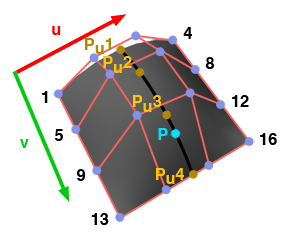
\includegraphics[width=0.5\textwidth]{bezier-surface.png}
    \caption{Будування поверхні Безьє}\label{fig:bezier-surface}
\end{figure}

Розглянемо графічний спосіб побудови кубічної поверхні Безьє з 16 контрольними точками. Спочатку ми будуємо 4 кубічні криві Безьє через контрольні точки 1-4, 5-8, 9-12, 13-16 використовуючи дійсне число $v$, далі використовуючи точки відповідних $v$ на отриманих кривих як контрольні точки наступної кривої будуємо наступну криву використовуючи дійсне число $u$, таким чином ми отримаємо поверхню побудованої з багатьох кривих, причому як ми все знаємо відрізок отриманий в останньому кроці при побудові кривої це дотична, якщо ми побудуємо поверхню будуючи криві по контрольним точкам 1, 5, 9, 13 і так далі до 4, 8, 12, 16, то ми отримаємо ще одну дотичну, але в деякому іншому напрямку, і якщо ми знайдемо векторний добуток отриманих дотичних, ми отримаємо нормаль до поверхні у данній точці.

...Обший вид...

\subsection{Бібліотека Visualization Library}

У ході роботи було знайдено таку біблиотеку, як Visualization Library. Це біблиотека написана на мові C++ і може використовуватись для графіки у 2D або 3D. Вона дозволяє моделювати різні види поверхонь, фрактали, та багато іншого.

Зробимо аналіз цієї бібліотеки.

\begin{itemize}
\item Бібліотека написана на мові C++, тобто це звужує кількість мов, що можуть використовувати цю бібліотеку.
\item Бібліотека самостійно реалізує свою матрицю та вектор, таким чином закривають можливість оптимізувати операції над матрицями. Більш того бібліотека не  використовує команди SSE, які дають приріст у швидкості, як це зроблено у бібліотеці CGLM.
\item Бібліотека вже не підтримується розробниками, останній внесення змін у код було 20 лютого 2020 року, у порівнянні з бібліотекою CGLM, яка активно розвивається.
\item Якщо подивитися на реалізацію кривих Безьє, то ми побачимо, що бібліотека не використовує матричний спосіб отримання вершин з поверхні Безьє, таким чином ми знову не можемо використати оптимізацію за допомогою команд SSE.
\item Також перерірено спосіб знаходження нормалей для поверхні, біблиотека знаходить нормалі по отриманим трикутникам при будуванні поверхні, хоча для поверхні Безьє існує значно швидший та дешевший спосіб знаходження нормалі, цей спосіб будується на знаходження похідних до кривої Безьє з різних сторін.
\end{itemize}

\section{Вимоги до розробленого програмного забезпечення}

Для розробки програмного забезпечення висунуто такі вимоги:
\begin{itemize}
\item Програмне забезпечення повинно мати відкритий вихідний код та ліцензію вільного програмного забезпечення.

Це дозволить будь якому досвідченому користувачу зкомпілювати програмне забезпечення під будь яку платформу та операційну систему, або навіть дасть можливість модифікувати код під свої потреби.

Також ліцензія повинна бути сумісна з ліцензіями використаних бібліотек. Загалом були використані бібліотеки CGLM, Nuklear, GLFW, uthash та прогрмний інтерфейс OpenGL. Перші біблиотеки CGLM та Nuklear використовують ліцензію MIT, бібліотека GLFW використовує ліцензію ZLib, а uthash -- ліцензію BSD. А програмний інтерфейс OpenGL має ліцензію подібну до ліцензії BSD. Усі ці ліцензії є сумісними з ліцензією LGPLv3, яка є подібною до GPL, але дозволяє використовувати програмне забезпечення у пропріетарних проектах.

\item Програмне забезпечення повинно працювати у режимі реального часу.

Саме таким чином було вибрано мову C та бібліотеку CGLM, які дозволяють досягти найбільшої швидкості роботи програми у порівнянні з іншими мовами програмуванні, причому практично не знижуючи швидкості розробки коду. Більш того CGLM автоматично компілюється з використанням SSE команд, якщо є така можливість, що ще дає приріст у швидкості.

\item Програмне забезпечення повинно дати можливість використання бібліотеки якомога більшому колу розробників.

Це ще одна причина вибору мови C, яку можна обернути у більшість мов програмування і таким чином програмне забезпечення зможуть використати і розробники, які не знають C, але знають деяку іншу мову програмування.

\item Програмне забезпечення повинно бути якомога простим та легким, та залежати від простих та легких бібліотек.

Програмне забезпечення повинно розроблятися по принципу KISS (акронім для ``Keep it simple, stupid''), що означає що проектування повинно бути якомога простішим. Таким чином можна уникнути багатьох помилок пов'язані з тим що неможливо розробник не може охопити структуру вихідного коду складного програмного забезпечення, а також таке програмне забезпечення має дуже малий розмір зкомпільованої програми, що підвищує легкість розповсюдження. І це третя причина чому було вибрано саме мову програмування C, яка має дуже простий синтаксис та просту структуру. А також саме тому було вибрано саме такий набір бібліотек, а загалом графічну бібліотеку Nuklear, яка має досить невеликий обсяг коду, приблизно 30 тисяч строк коду разом з коментарями.
\end{itemize}


%\section{Опис програмного забезпечення}

%\subsection{Опис модулів програми}

%\section{Огляд роботи програми}

\section*{ВИСНОВКИ}
\addcontentsline{toc}{section}{ВИСНОВКИ}
У ході курсової роботи були отримані такі результати:

\begin{itemize}
\item досліджено математичні моделі динамічних гладких об'єктів та вибрано оптимальний спосіб для розв'язання поставленої задачі,
\item розроблене програмне забезпечення для відображення динамічних об'єктів,
\item частково розроблене програмне забезпечення для створення або редагування динамічних об'єктів.
\end{itemize}

\begin{thebibliography}{9}
\bibitem{} Офіційний сайт Міністерства освіти та науки України: http://mon.gov.ua/
\bibitem{} СТП-02066747-009-01. Стандарт Дніпропетровського національного університету. Методика виконання випускних, курсових та дипломних проектів (робіт). Структура, правила оформлення та порядок узгодження і затвердження. Затверджено ректором ДНУ 31.10.2001 р.
\bibitem{} СТП-02066747-010-01. Стандарт Дніпропетровського національного університету. Організація та проведення дипломування. Затверджено ректором ДНУ 1.11.2001 р.
\bibitem{} http://www.dnu.dp.ua/docs/obgovorennya/Polozhennya\_Antiplagiat\_2016.doc
\bibitem{porev} Порев. В.Н. Компъютерная графика -- СПб: БХВ-Петербург, 2002 -- 432 c.
\bibitem{nikulin} Никулин Е. A. Компъютерная геометрия и алгоритмы машинной графики. -- СПб: БХВ-Петербург, 2003 -- 560 c.
\end{thebibliography}

%\end{document}
\section*{Додаток A. Лістинг програми}
\addcontentsline{toc}{section}{Додаток A. Лістинг програми}
\tiny

\end{document}
